\section{Features Guide}
The following section contains the list of all the allowed operations that the different types of user can perform inside \app. \\
Please note that, due to time reasons, not all the features are currently implemented, but they will be implemented in a short time and this section will be so updated. These features will be marked by a * near their names.

\subsection{Users' types}
The common use of the application will involve different types of users, which can be represented by the following hierarchy, from the one that has fewer permissions (at the top) to the one with the most permissions (at the bottom):
\begin{itemize}
	\item \textbf{Common user}, also called \textbf{user}.
		  This kind of user does nothing else than interacting with an already-created list, performing common operations. The operations that this kind of user can perform will be marked with an \texttt{[U]} near their name;
	\item \textbf{Permissions-granted user}, also called \textbf{editor}.
		  This kind of user has all the above permissions, plus he can add or remove items to the list. All the operations that he can perform will be marked with an \texttt{E} near their name;
	\item \textbf{Creator of the list}, also called \textbf{creator}
		  This kind of user is the user that creates a list and so can perform some special actions on it. The operation that this kind of user can perform are marked with a \texttt{[C]} near their name.
\end{itemize}

\newpage
\subsection{[U] Creating a list}
In order to create a list just click on the list button that is present on the right-side bar of the chat.

% Inserire immagine del bottone
\begin{figure}[H]
  \centering 
  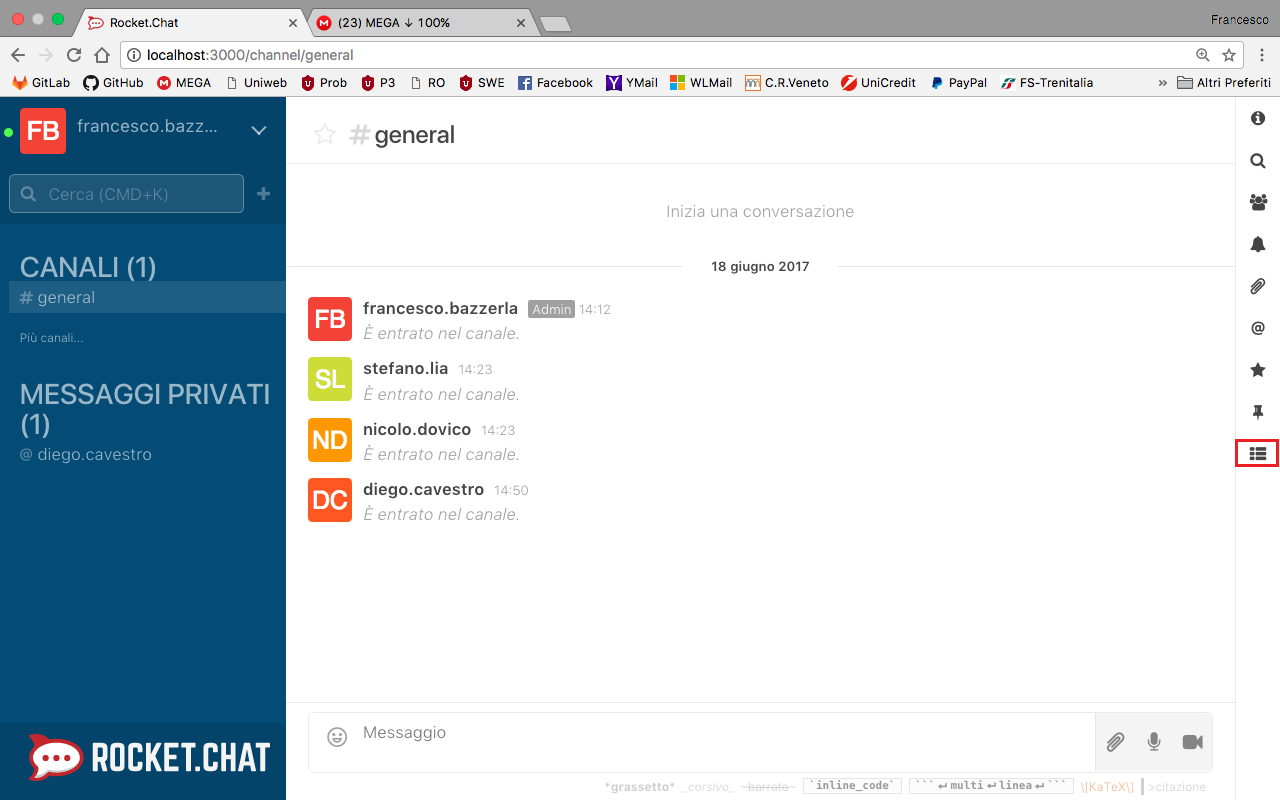
\includegraphics[width=\textwidth]{Sections/3-HowToUse/Images/button_list_create.png}
  \caption{Bubble creation button.}
\end{figure}

This will open the following screen, where you can input all the information that you want about the list, reminding that the only \textbf{required option} is the list's title.

\begin{figure}[H]
  \centering 
  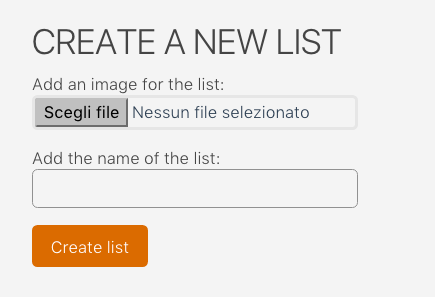
\includegraphics[width=\textwidth]{Sections/3-HowToUse/Images/list_create.png}
  \caption{Empty bubble creation input screen.}
\end{figure}

Once that all the information are input, in order to create the list just click on the \textit{"Create"} button, which will create the bubble as shown below.

\begin{figure}[H]
  \centering 
  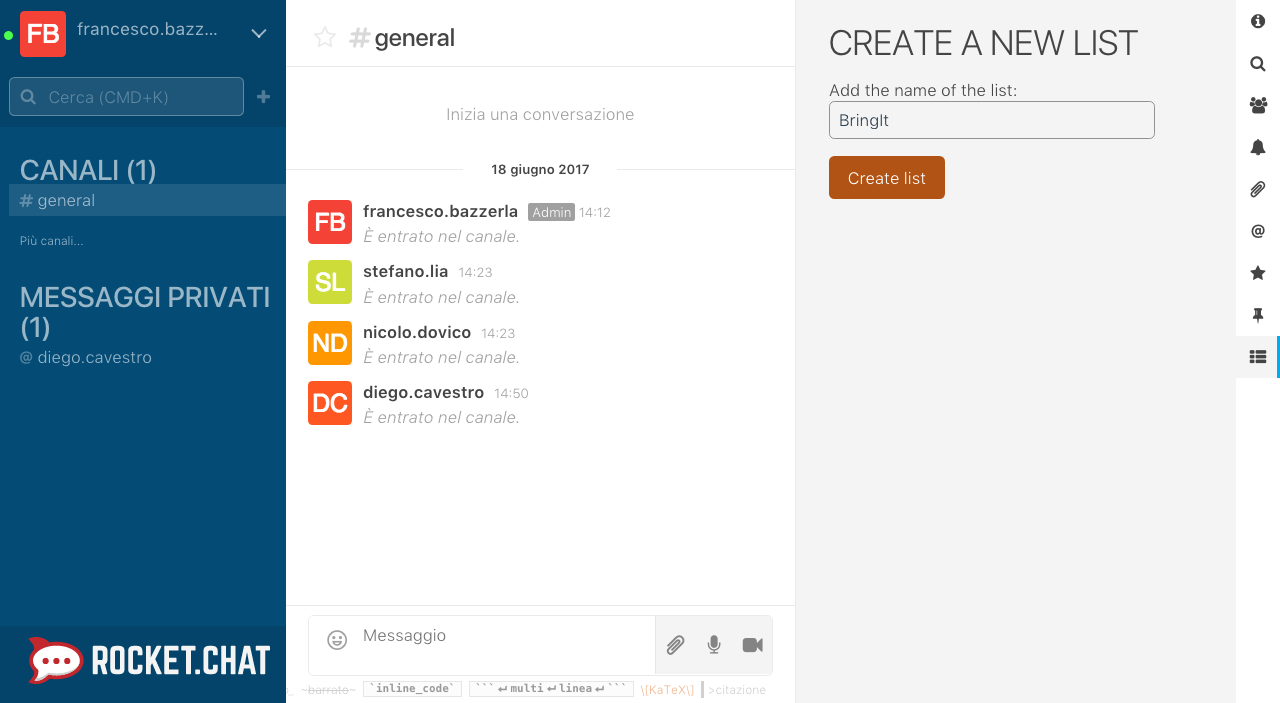
\includegraphics[width=\textwidth]{Sections/3-HowToUse/Images/list_create_filled.png}
  \caption{Filled bubble creation input screen.}
\end{figure}

% Inserire immagine della bolla creata
\begin{figure}[H]
  \centering 
  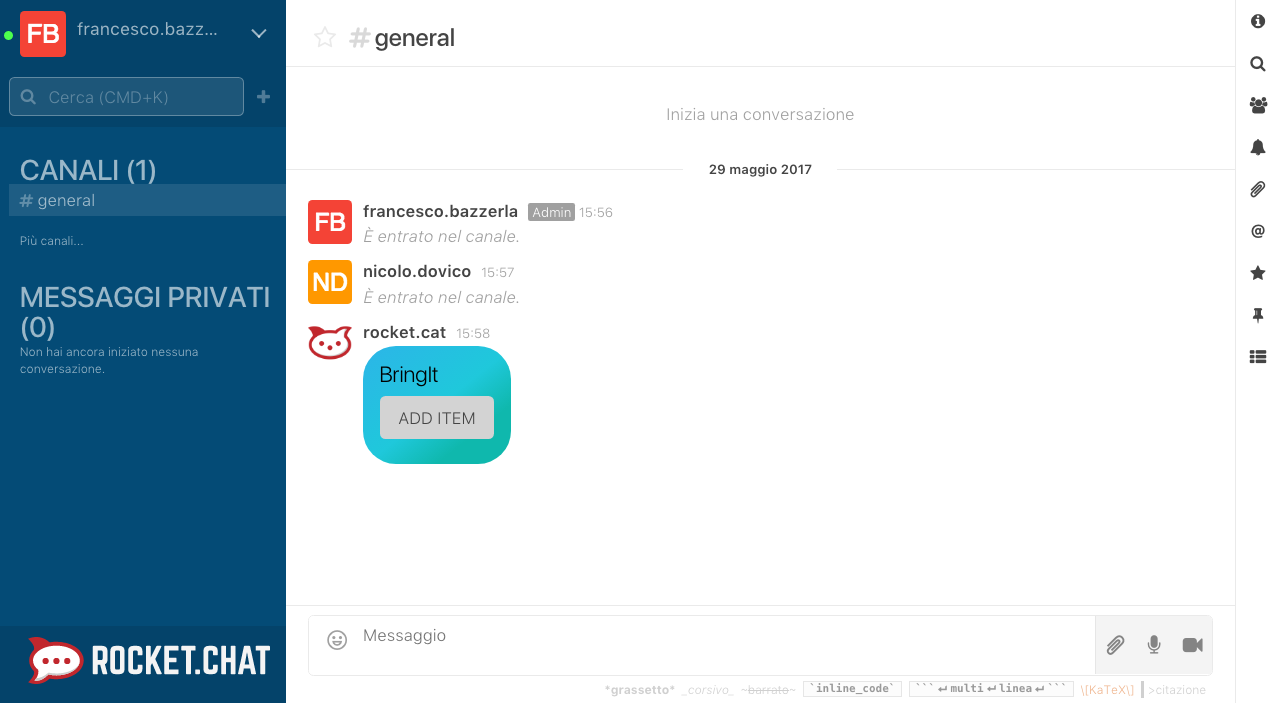
\includegraphics[width=\textwidth]{Sections/3-HowToUse/Images/bubble_empty.png}
  \caption{Created bubble which represents the list.}
\end{figure}
\newpage
\subsection{[U] Deleting a list}
In order to delete a list, hover above the bubble that represents the list, and click on the options button.

\begin{figure}[H]
  \centering 
  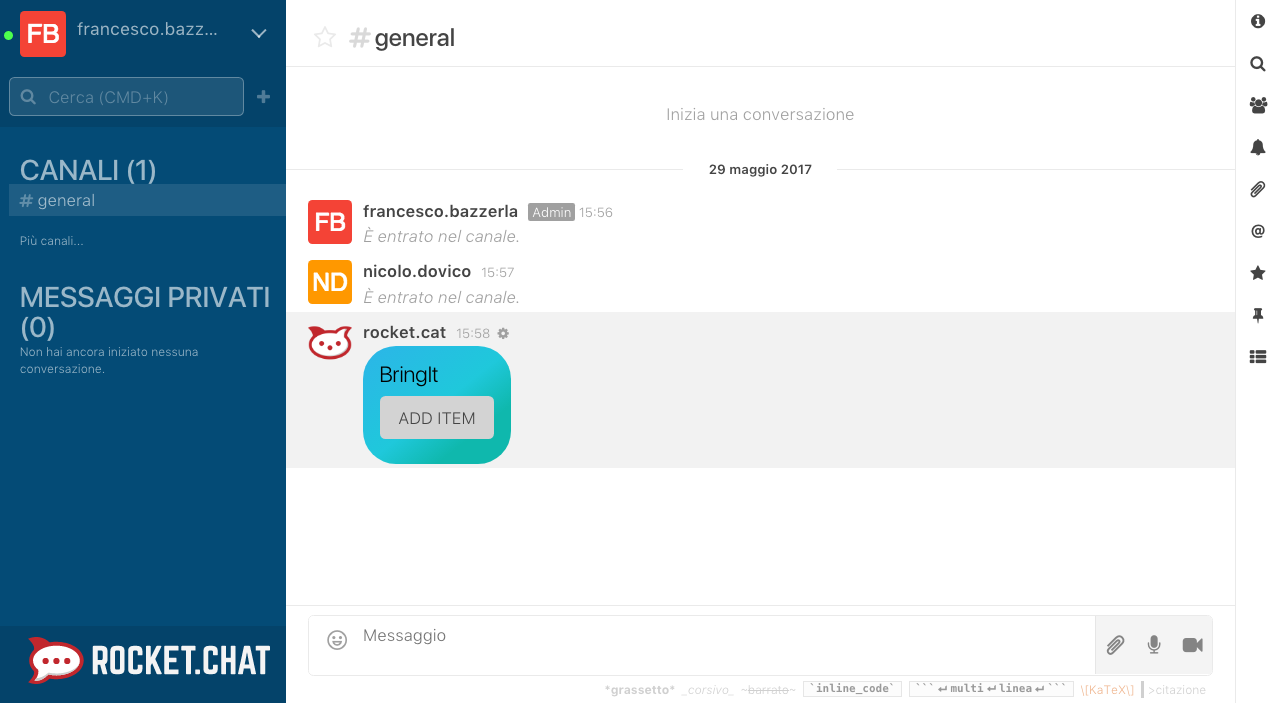
\includegraphics[width=\textwidth]{Sections/3-HowToUse/Images/bubble_options_button.png}
  \caption{Button to show the available list's actions.}
\end{figure}

From the options that appear, click on the one to delete the list, represented by an "X".

% Inserire immagine del bottone
\begin{figure}[H]
  \centering 
  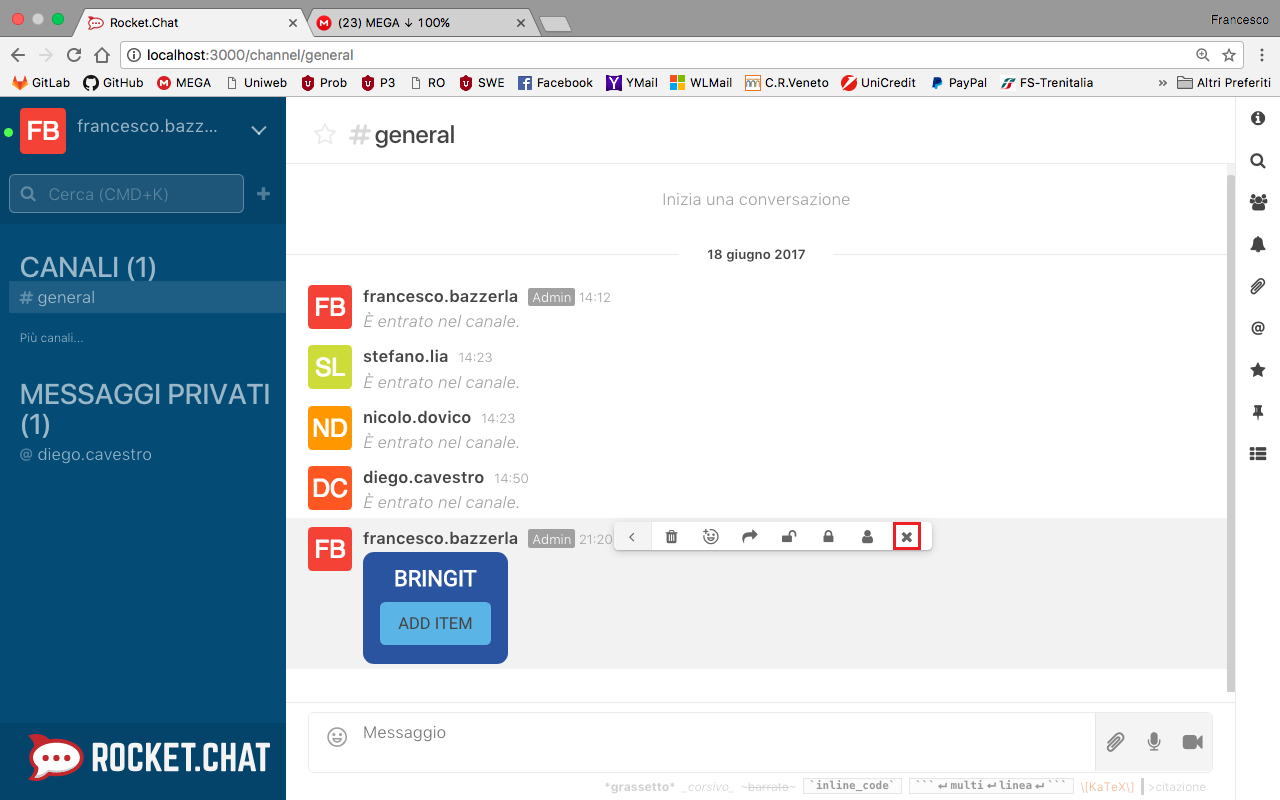
\includegraphics[width=\textwidth]{Sections/3-HowToUse/Images/bubble_option_delete.png}
  \caption{Button to delete a list.}
\end{figure}

This will open the following popup, asking you if you want to confirm the deletion.

\begin{figure}[H]
  \centering 
  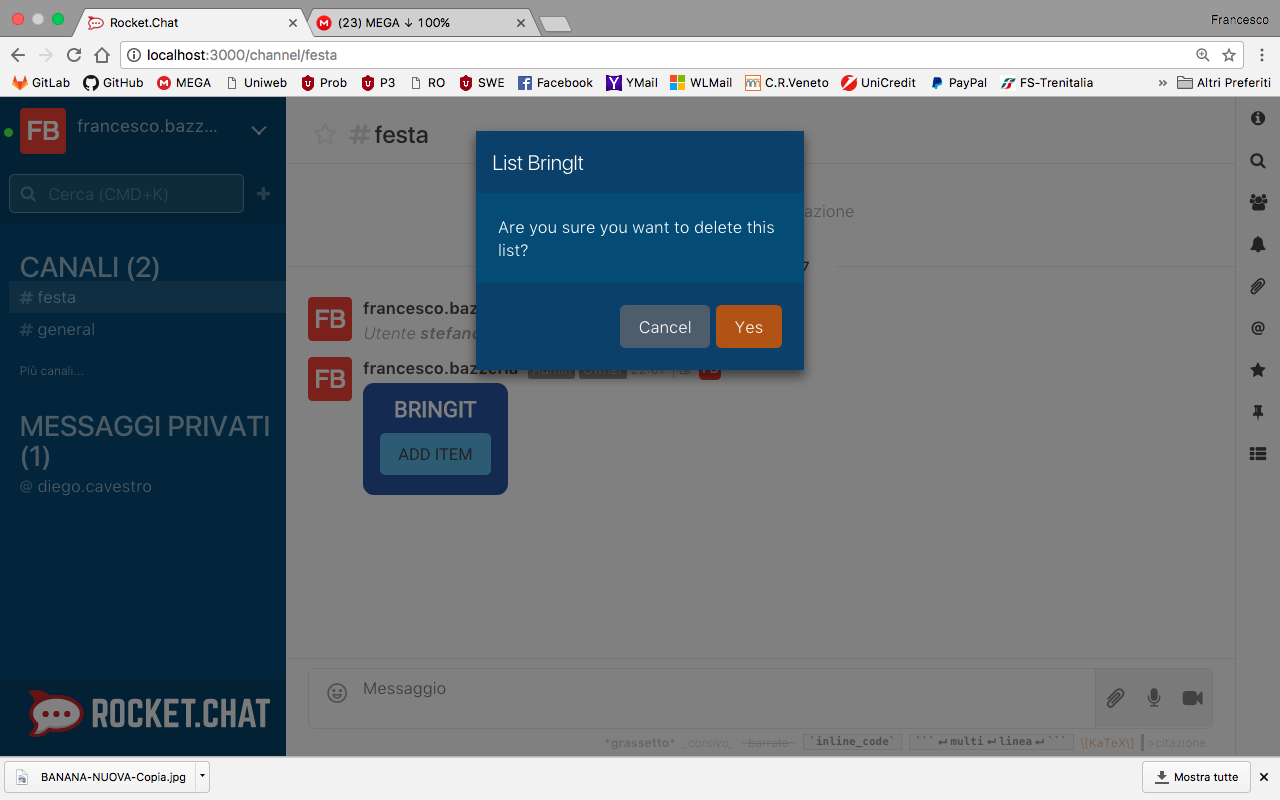
\includegraphics[width=\textwidth]{Sections/3-HowToUse/Images/popup_delete_confirm.png}
  \caption{Popup to confirm the deletion of a list.}
\end{figure}

Once you click on "Yes", the list will be deleted, showing you the popup telling that the deletion has been successful.

\begin{figure}[H]
  \centering 
  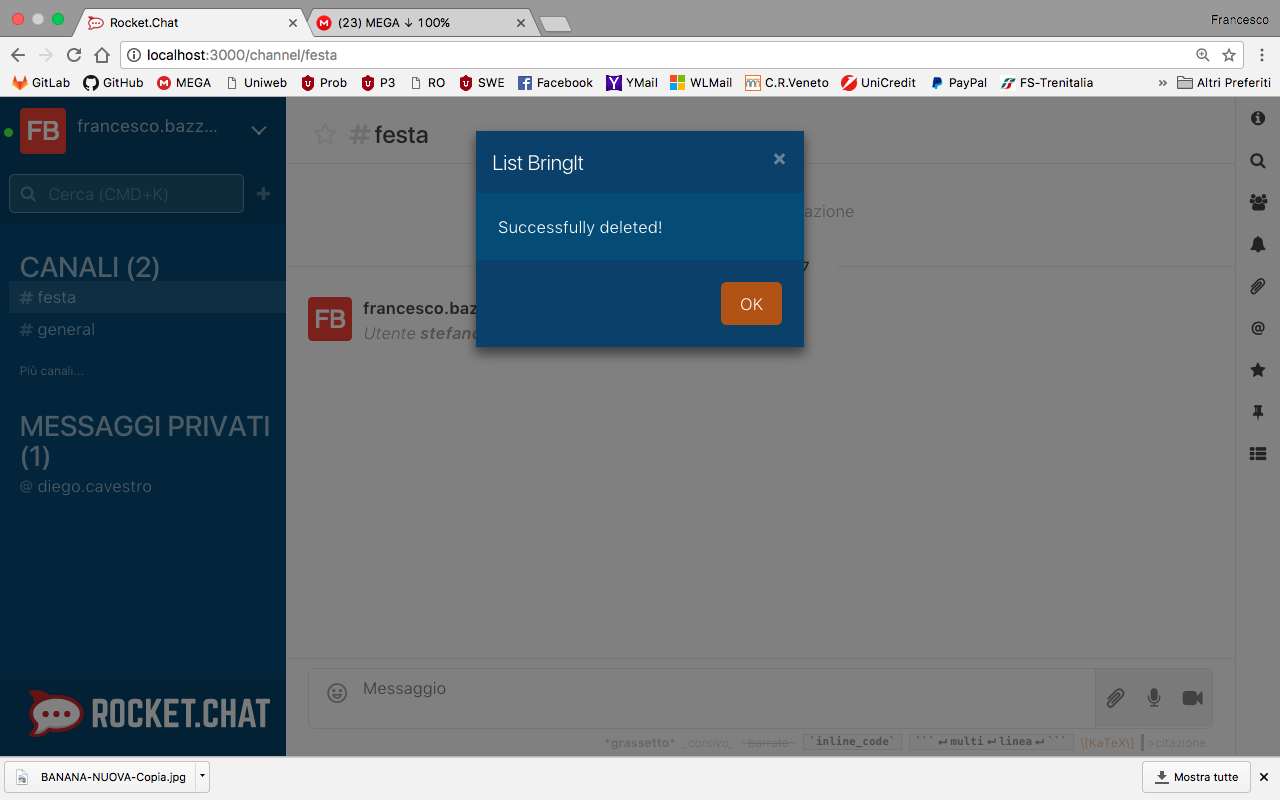
\includegraphics[width=\textwidth]{Sections/3-HowToUse/Images/popup_delete_success.png}
  \caption{Popup indicating the success of the deletion of a list.}
\end{figure}

In order to delete the bubble that represents that list, you also have to confirm the operation from the following popup that will be opened.

% Inserire immagine della bolla creata
\begin{figure}[H]
  \centering 
  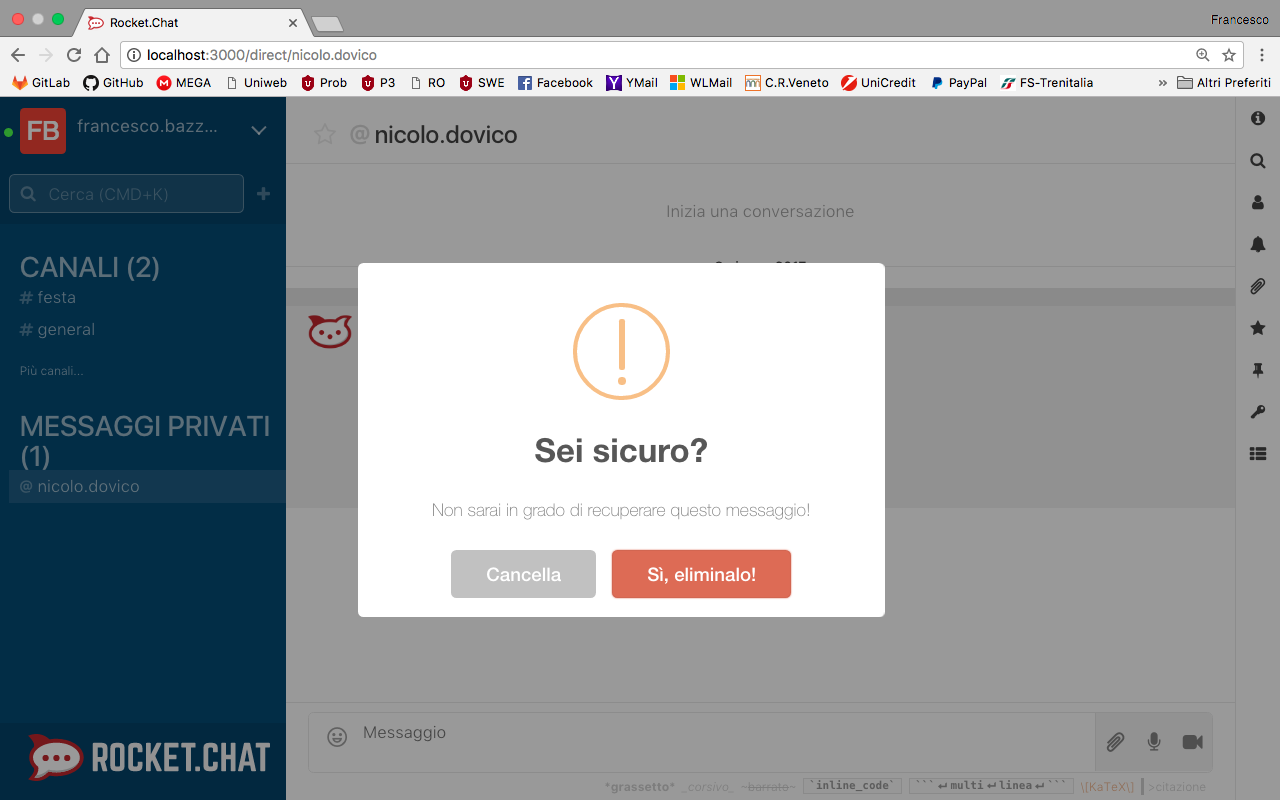
\includegraphics[width=\textwidth]{Sections/3-HowToUse/Images/popup_delete_message.png}
  \caption{Popup asking to delete the bubble representing a list.}
\end{figure}

Once that \textit{"Yes, delete it!"} will be clicked, the list will be deleted.

\newpage
\subsection{[E] Adding an item to the list}
In order to add an item to the list, just click on the proper button that is present on the bubble that represents the list itself.

% Immagine della bolla con il bottone per aggiungere un oggetto
\begin{figure}[H]
  \centering 
  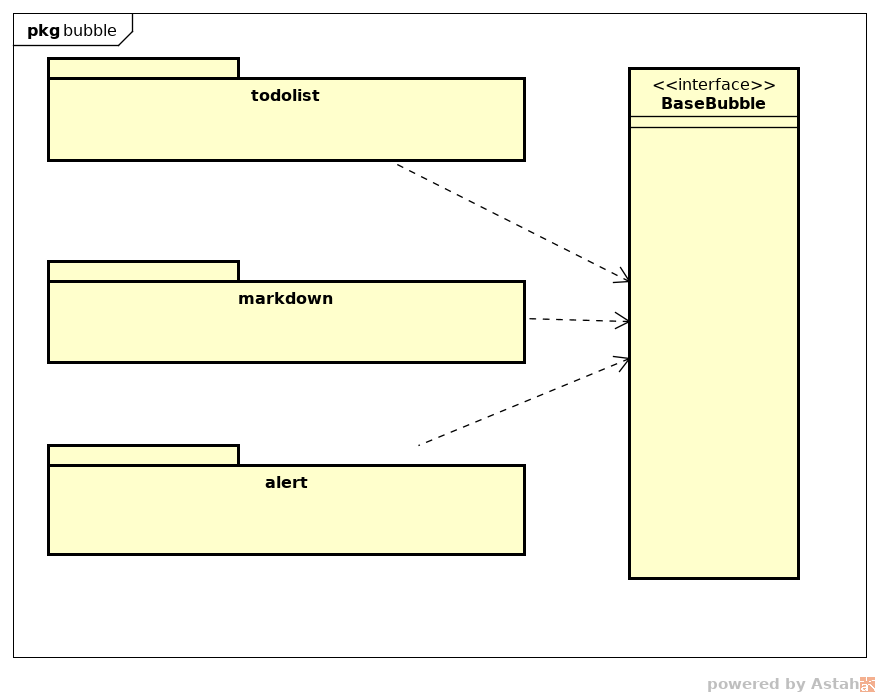
\includegraphics[scale=0.3]{Sections/3-HowToUse/Images/bubble.png}
  \caption{Bubble with the button to add an item inside.}
\end{figure}

This will open the following screen, where you can input all the information about the item that needs to be added to the list. \\

% Immagine della schermata per inserimento dati oggetto
\begin{figure}[H]
  \centering 
  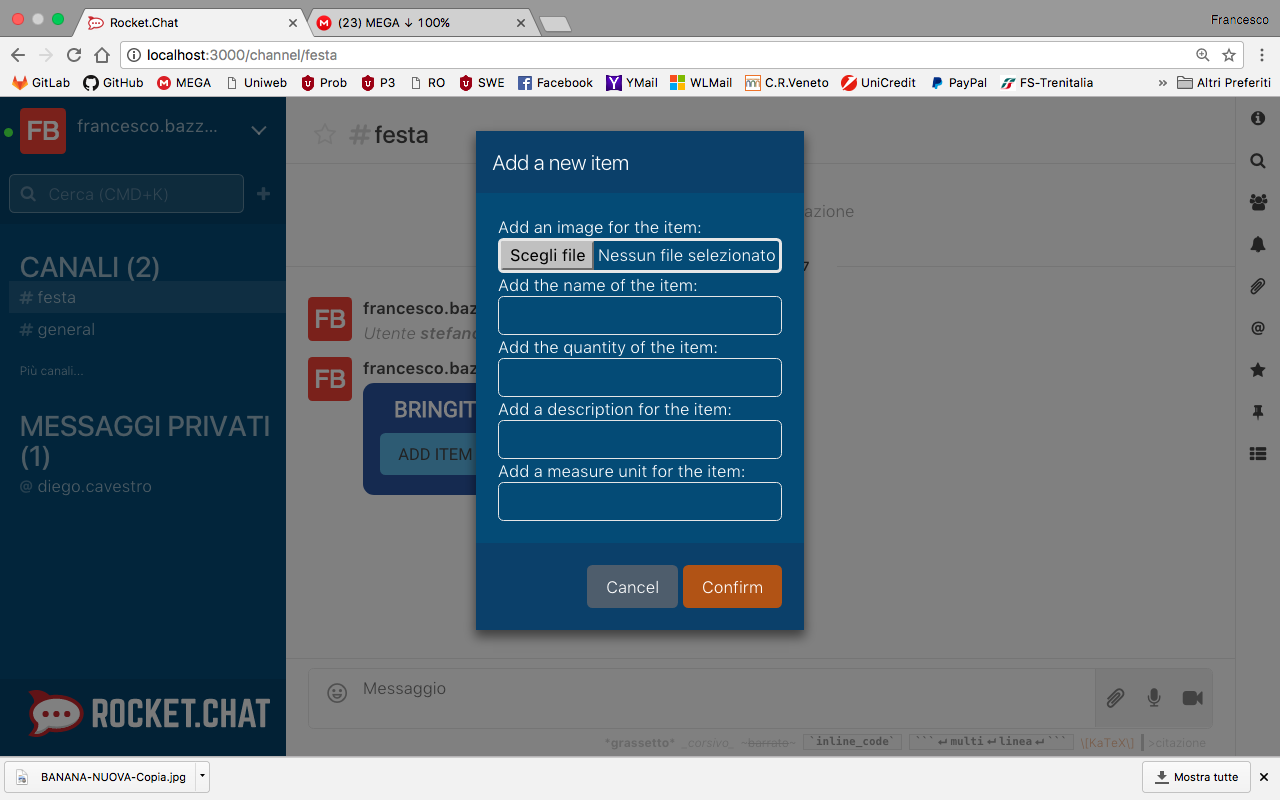
\includegraphics[scale=0.5]{Sections/3-HowToUse/Images/item_add.png}
  \caption{Item information input screen.}
\end{figure}

Once that all the data have been input, in order to add the item just click on the \textit{"Add"} button, which will add the item to the list.

% Immagine della bolla con il nuovo oggetto aggiunto
\begin{figure}[H]
  \centering 
  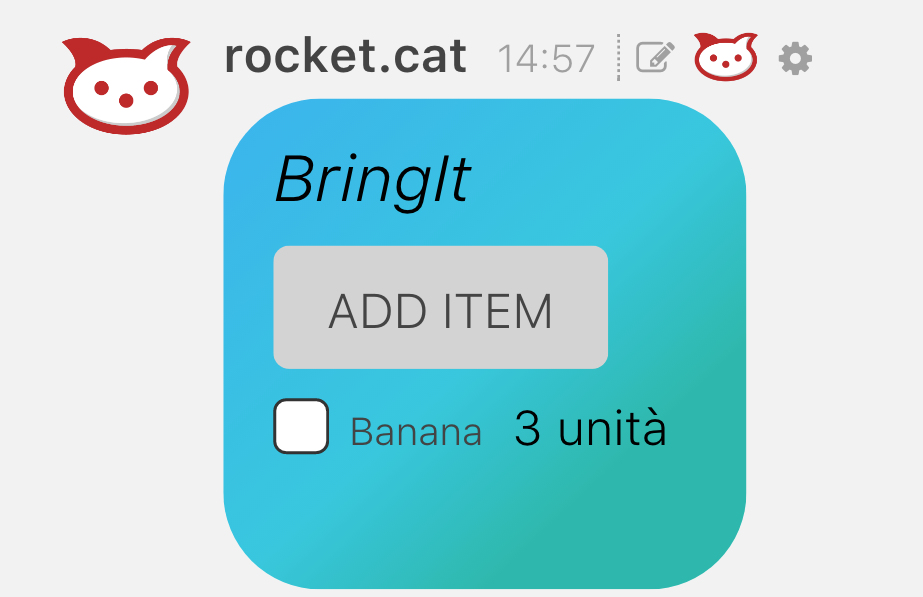
\includegraphics[scale=0.3]{Sections/3-HowToUse/Images/bubble_with_item.png}
  \caption{Bubble with the new item added.}
\end{figure}
\subsection{[E] Editing an item *}
In order to edit the information of an item inside the list, just long click the item that you want to edit, opening the following screen.

% Immagine della schermata di edit dei dati di un oggetto
\begin{figure}[H]
  \centering 
  
\includegraphics[width=\textwidth]{Sections/3-HowToUse/Images/example.jpeg}
  \caption{Item information editing screen.}
\end{figure}

Once you have modified all the information that you want, just click on the \textit{"Save"} button, which will save the edits you have performed.

% Immagine della bolla con l'oggetto modificato
\begin{figure}[H]
  \centering 
  
\includegraphics[width=\textwidth]{Sections/3-HowToUse/Images/example.jpeg}
  \caption{Bubble with the edited item inside.}
\end{figure}
\newpage
\subsection{[E] Removing an item from the list}
In order to remove an item from the list, just long click on the item that you want to remove. This will open the following popup showing the item's details.

\begin{figure}[H]
  \centering 
  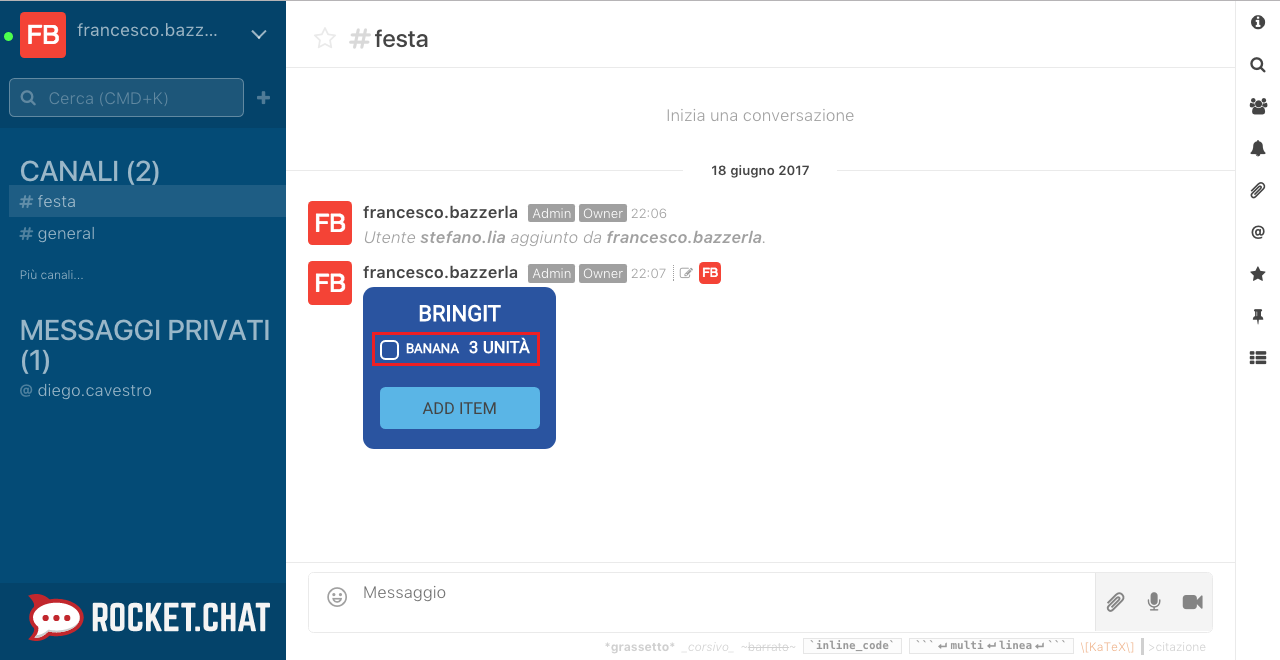
\includegraphics[width=\textwidth]{Sections/3-HowToUse/Images/bubble_item_to_delete.png}
  \caption{Popup showing the details of an item.}
\end{figure}

\begin{figure}[H]
  \centering 
  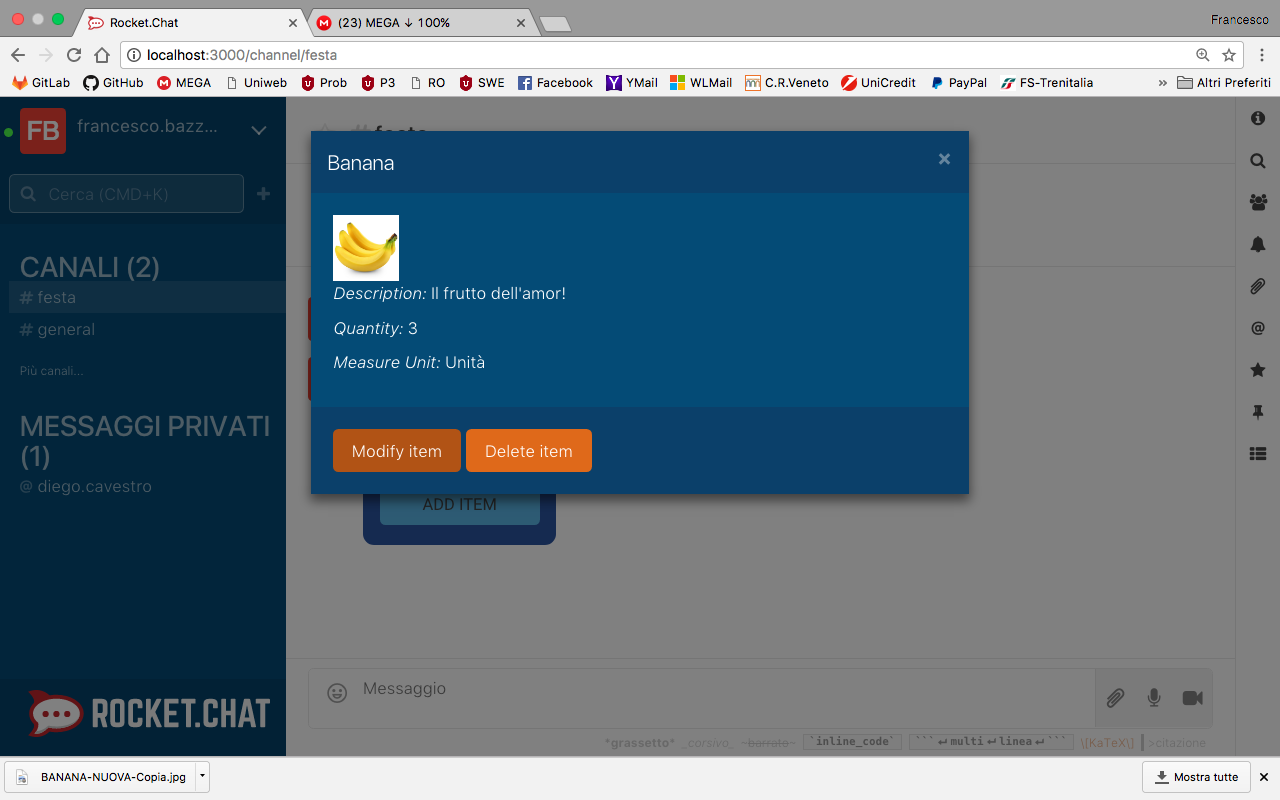
\includegraphics[width=\textwidth]{Sections/3-HowToUse/Images/item_details.png}
  \caption{Popup showing the details of an item.}
\end{figure}

To delete the item, just click on the \textit{"Delete"} button.

\begin{figure}[H]
  \centering 
  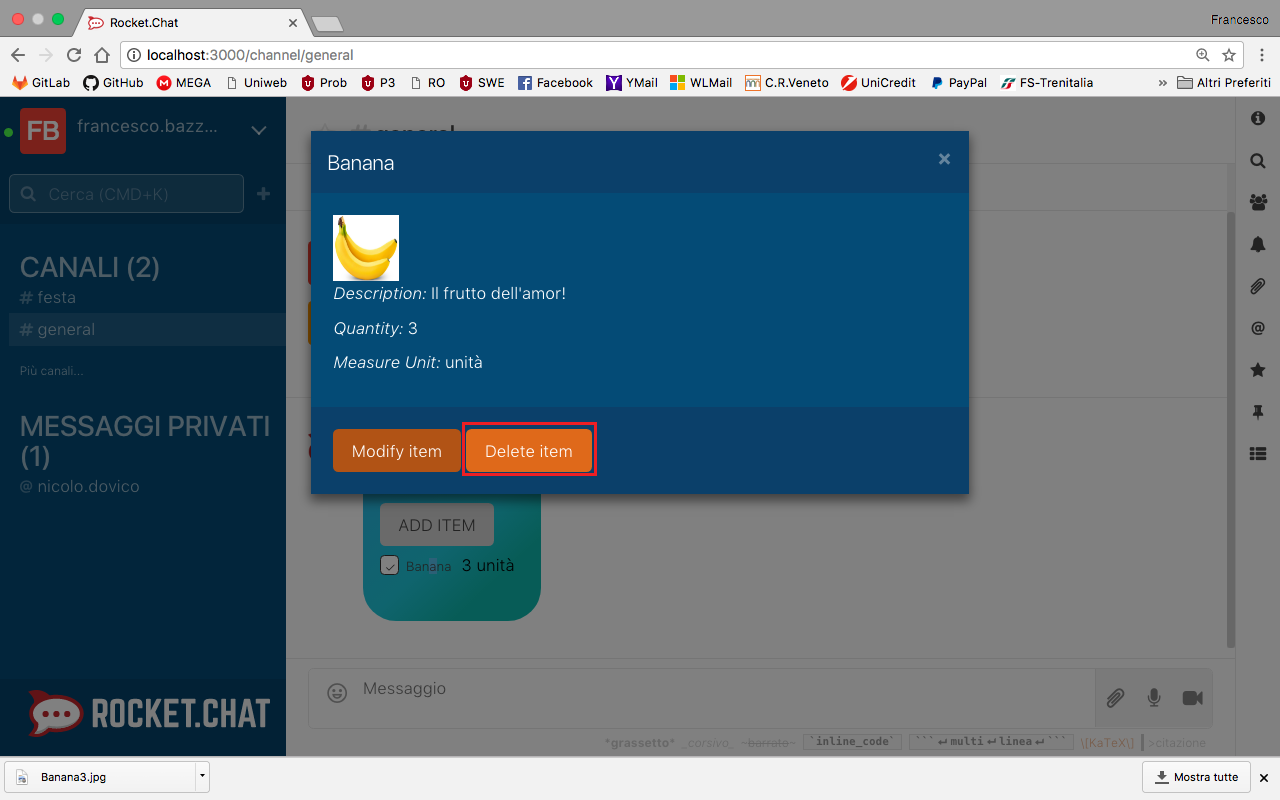
\includegraphics[width=\textwidth]{Sections/3-HowToUse/Images/popup_item_delete.png}
  \caption{Button to delete an item from a list.}
\end{figure}

\begin{figure}[H]
  \centering 
  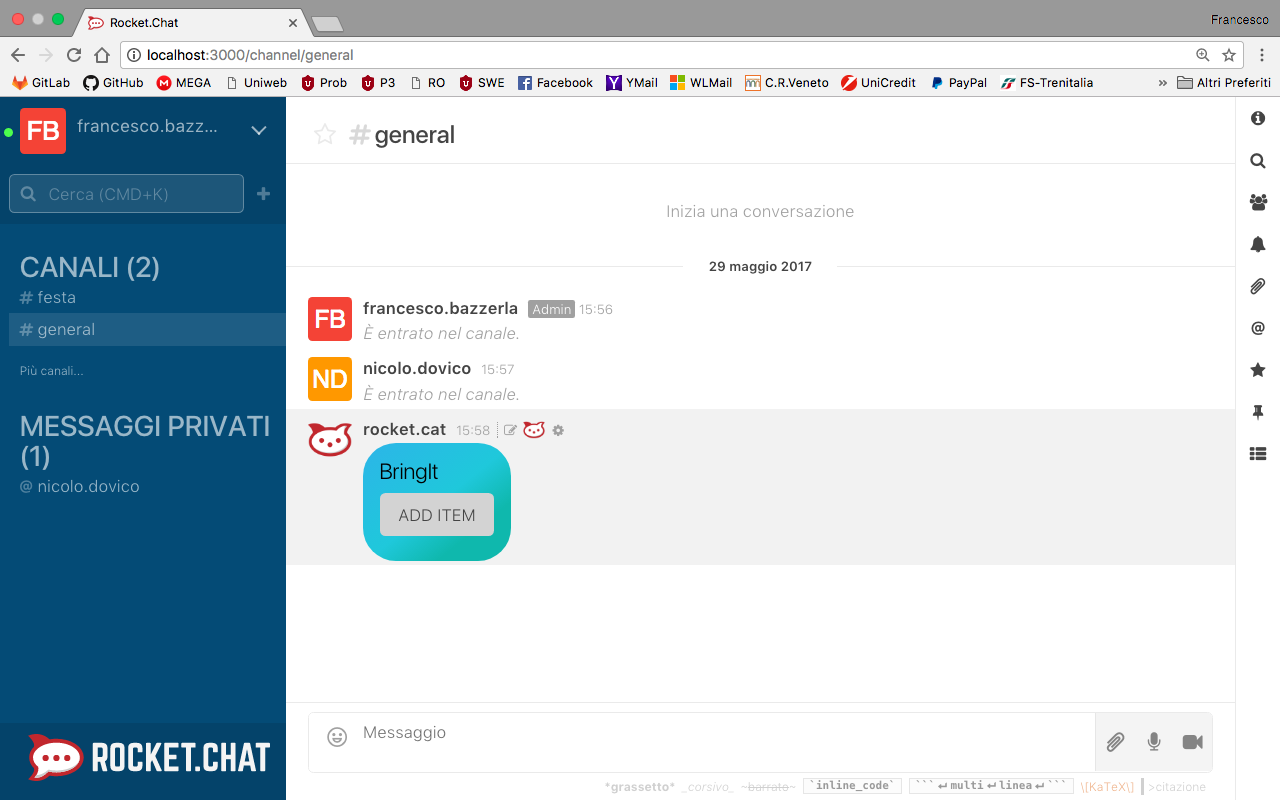
\includegraphics[width=\textwidth]{Sections/3-HowToUse/Images/bubble_item_deleted.png}
  \caption{Bubble with the deleted item.}
\end{figure}

\newpage
\subsection{[C] Sharing a list with a group}
In order to share a list with a group, hover on top of the \termine{bubble} that represents the list and click on the gear icon.

\begin{figure}[H]
  \centering 
  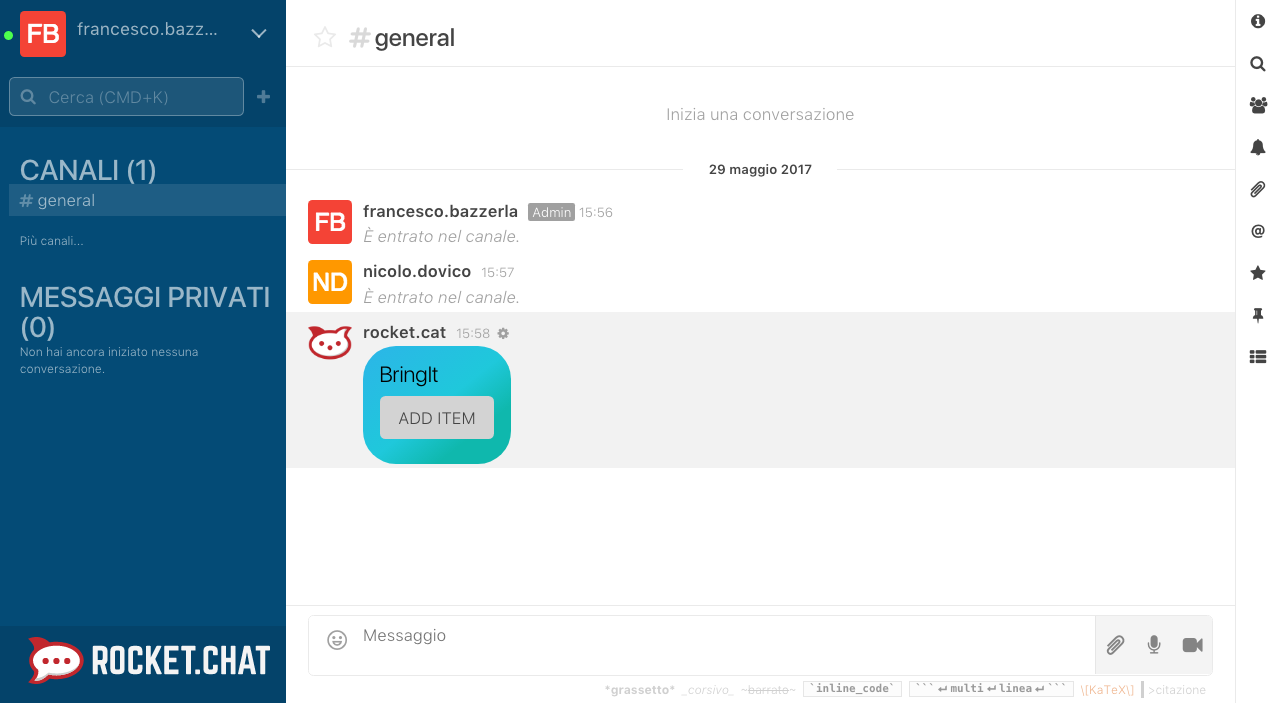
\includegraphics[width=\textwidth]{Sections/3-HowToUse/Images/bubble_options_button.png}
  \caption{Button to show the available list's actions.}
\end{figure}

From the various options that are available, click on the one with the sharing icon.

\begin{figure}[H]
  \centering 
  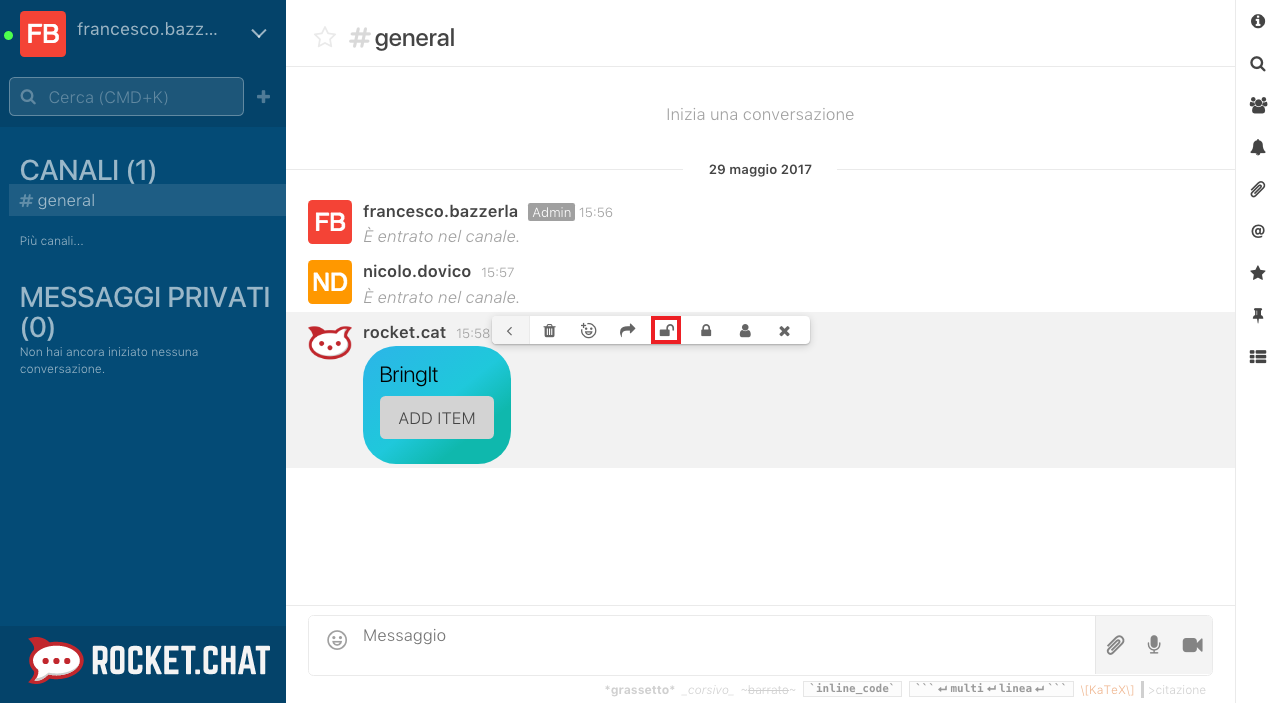
\includegraphics[width=\textwidth]{Sections/3-HowToUse/Images/bubble_option_share_group.png}
  \caption{Button to share the list with a specific group.}
\end{figure}

Once that the option has been clicked, the following popup will appear, showing the list of all the group that the list can be shared to.

\begin{figure}[H]
  \centering 
  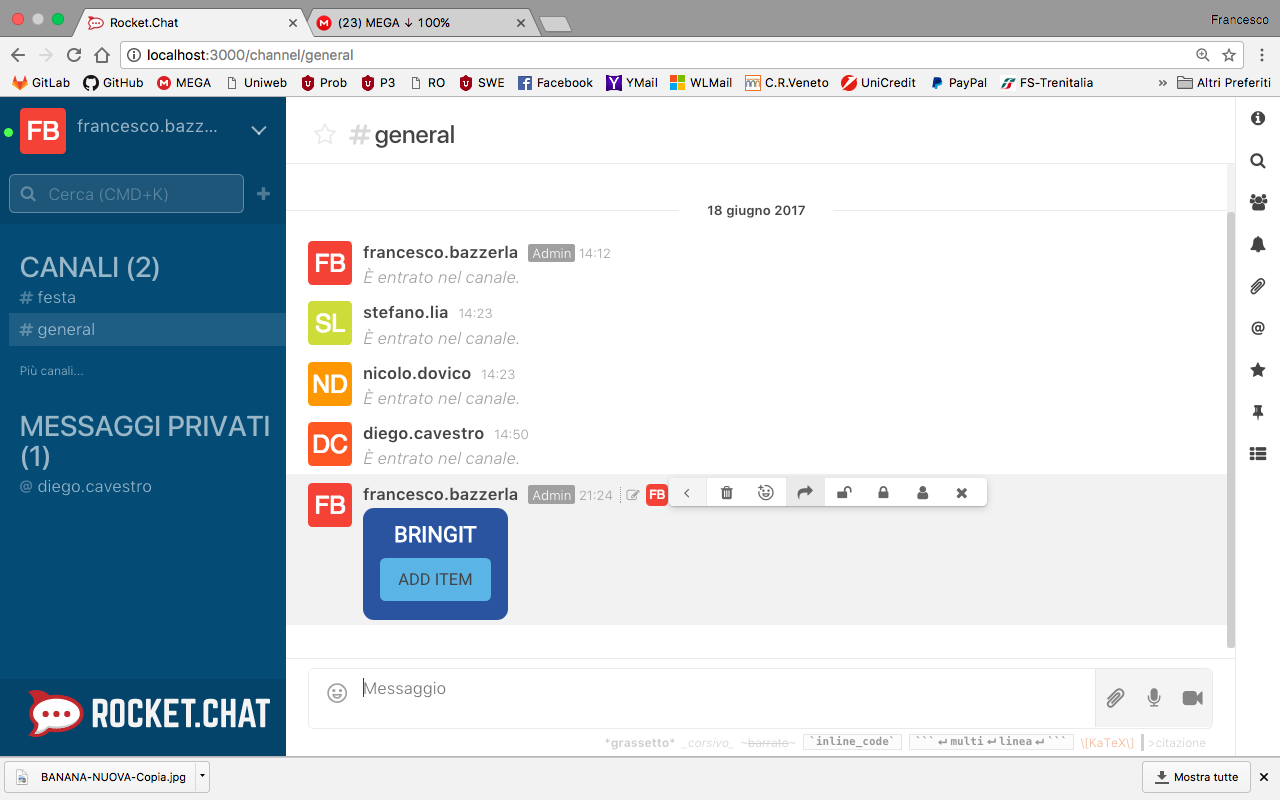
\includegraphics[width=\textwidth]{Sections/3-HowToUse/Images/share_group_channel.png}
  \caption{Popup showing the list of all the groups to which is possible sharing a list.}
\end{figure}

Now, select the group you want share the list with and then click on \textit{"Share"}. \\
This will open a new popup, letting you choose to which user you want to grant the \textbf{editor} permission. Once you have chose to which users to grant the permissions, click on \textit{"Ok"}.

\begin{figure}[H]
  \centering 
  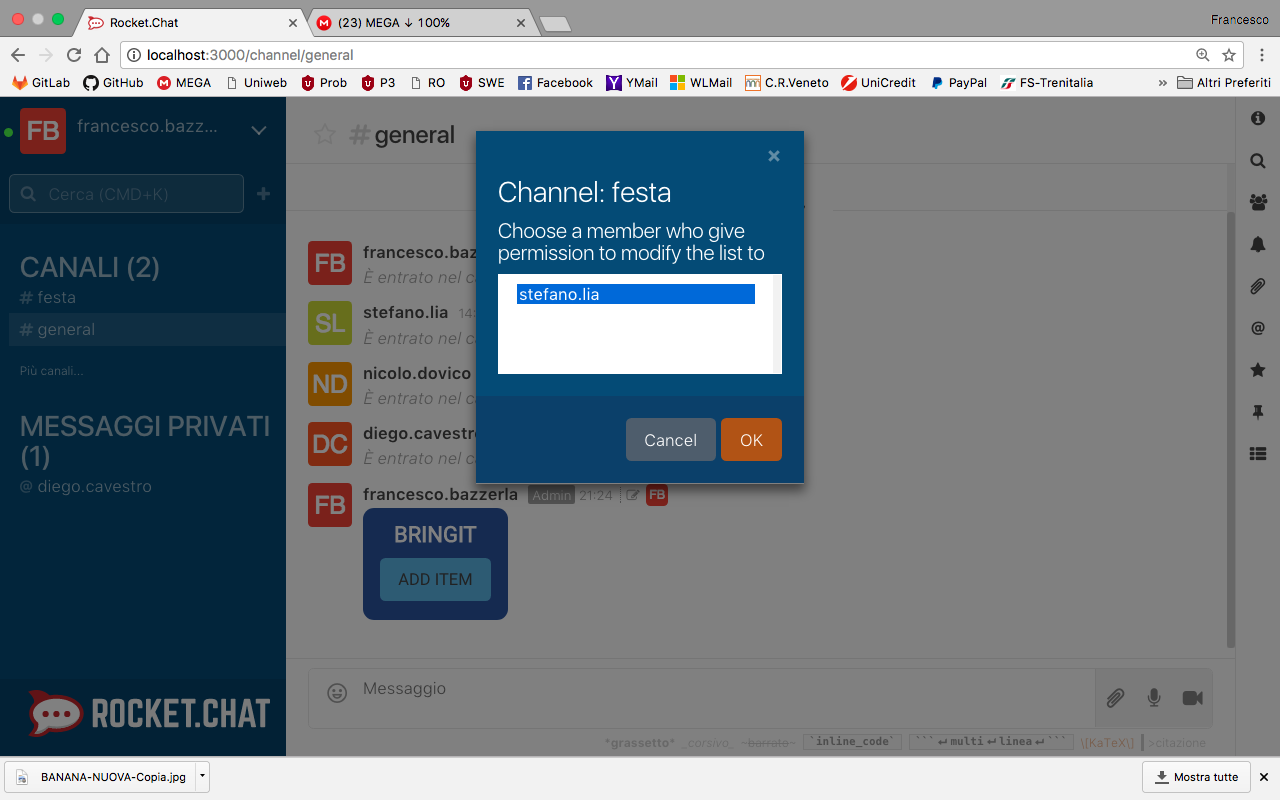
\includegraphics[width=\textwidth]{Sections/3-HowToUse/Images/share_group_user.png}
  \caption{Popup to grant the editor permission to users inside the group.}
\end{figure}

Note that, if there are no users you can share the list with, an error will be shown.

\begin{figure}[H]
  \centering 
  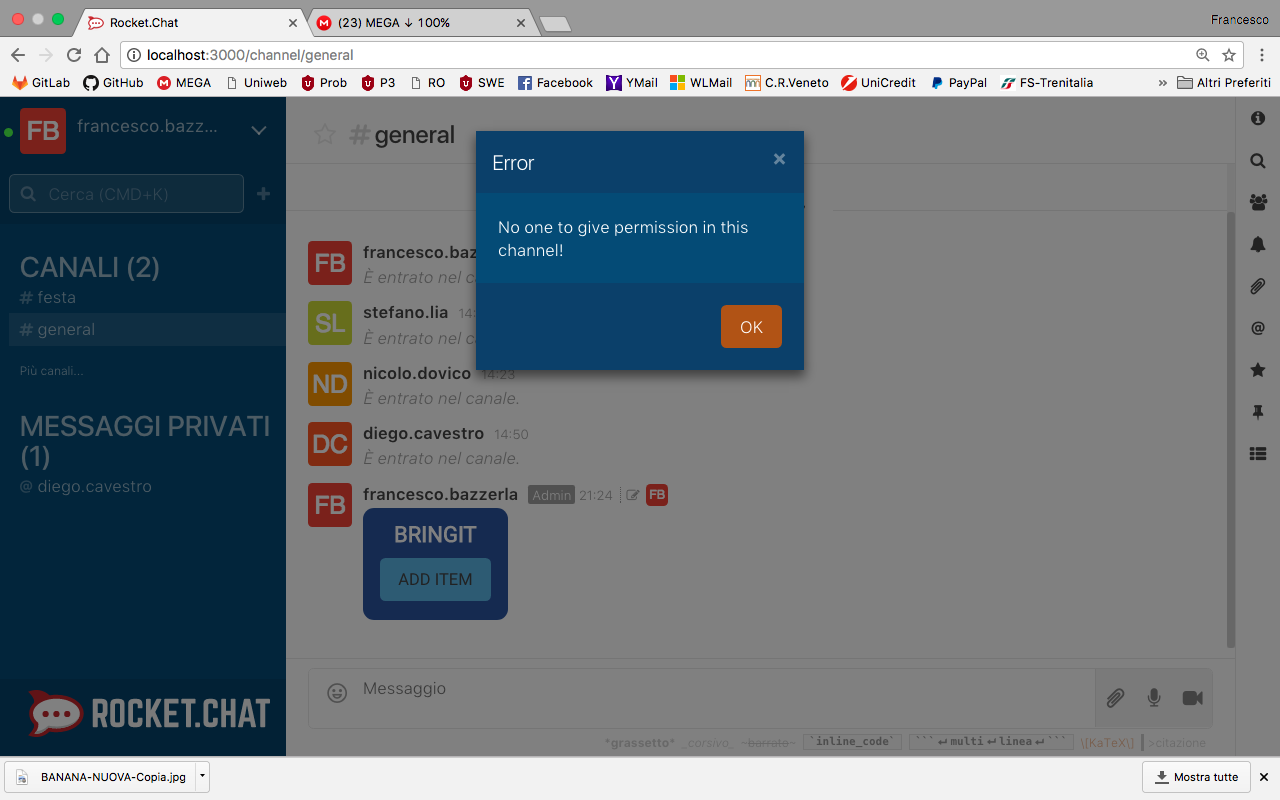
\includegraphics[width=\textwidth]{Sections/3-HowToUse/Images/popup_permission_give_error.png}
  \caption{Error shown if there are no users it's possible to share the list with.}
\end{figure}

Once that the sharing has been completed successfully, a message will be sent inside the proper channel


\begin{figure}[H]
  \centering 
  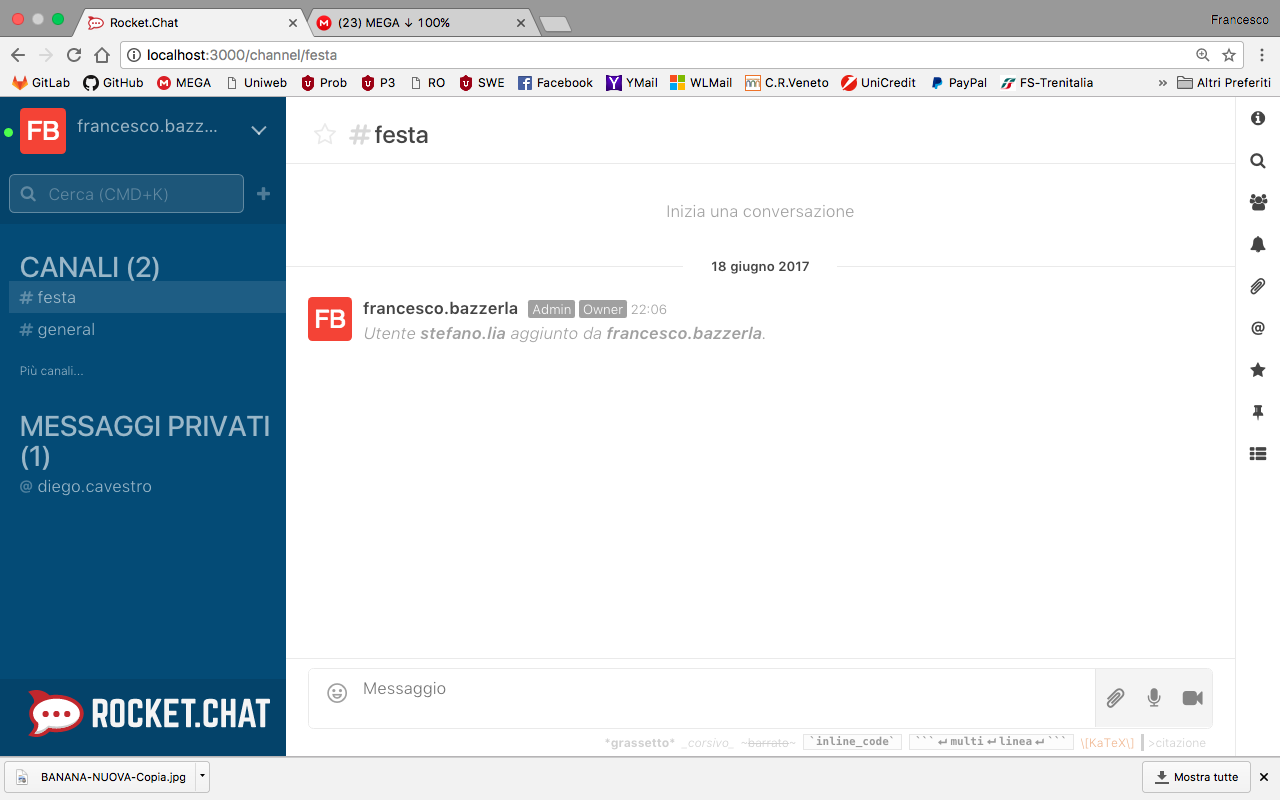
\includegraphics[width=\textwidth]{Sections/3-HowToUse/Images/share_group_before.png}
  \caption{Channel before the sharing of the list.}
\end{figure}

\begin{figure}[H]
  \centering 
  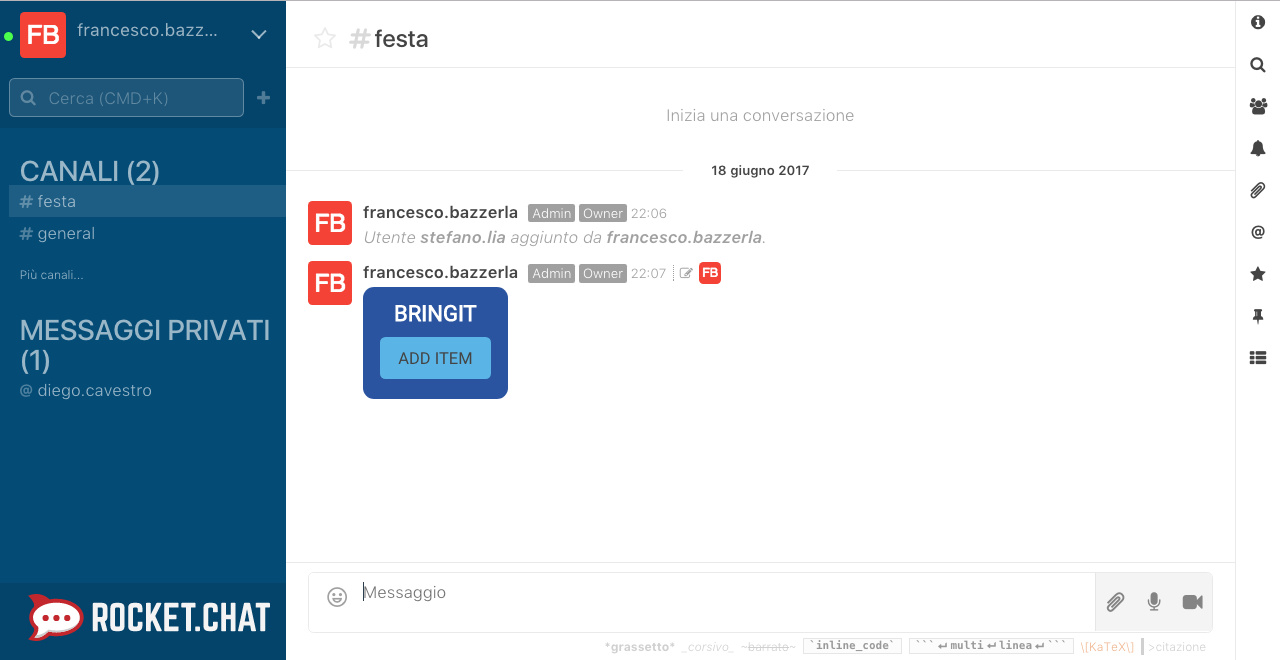
\includegraphics[width=\textwidth]{Sections/3-HowToUse/Images/share_group_after.png}
  \caption{Channel after the sharing of the list.}
\end{figure}
\newpage
\subsection{[C] Sharing a list with a user}
In order to share a list with a user, hover on top of the \termine{bubble} that represents the list and click on the gear icon.

\begin{figure}[H]
  \centering 
  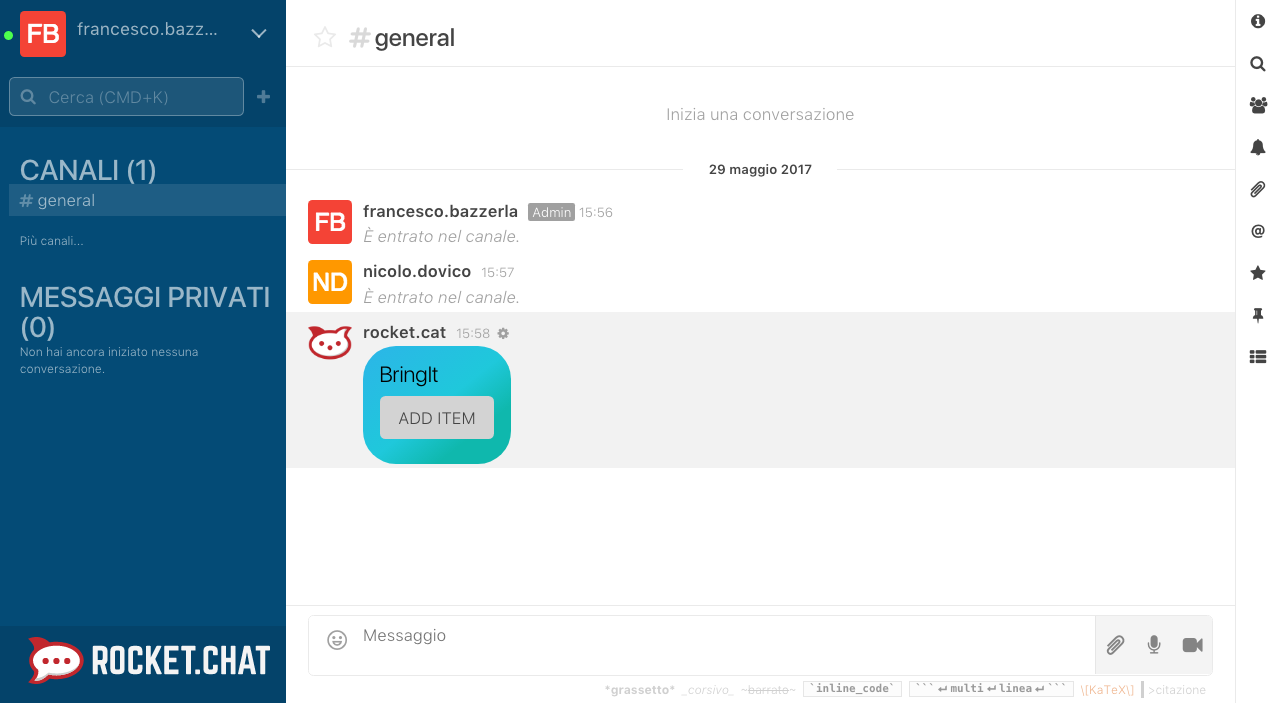
\includegraphics[width=\textwidth]{Sections/3-HowToUse/Images/bubble_options_button.png}
  \caption{Button to show the available list's actions.}
\end{figure}

From the various options that are available, click on the one with the user icon.

\begin{figure}[H]
  \centering 
  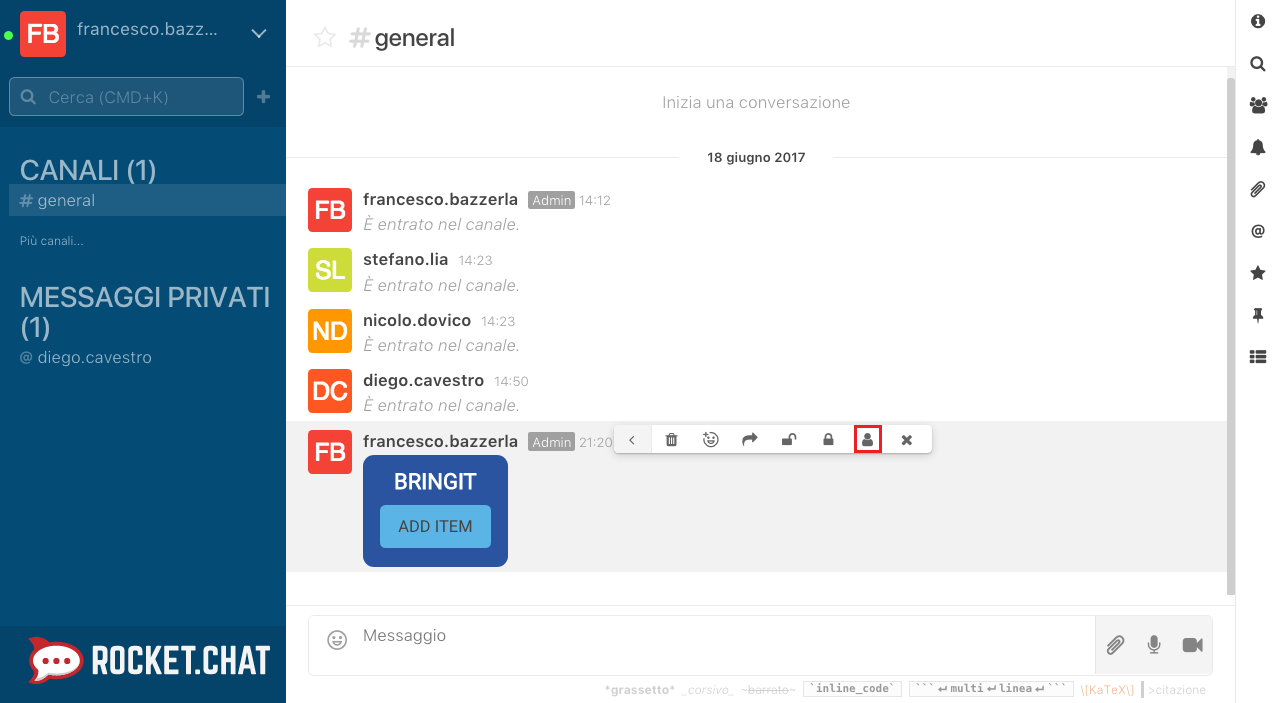
\includegraphics[width=\textwidth]{Sections/3-HowToUse/Images/bubble_option_share_user.png}
  \caption{Button to share the list with a specific user.}
\end{figure}

Once that the option has been clicked, the following popup will appear, showing the list of all the item that the list can be shared to.

\begin{figure}[H]
  \centering 
  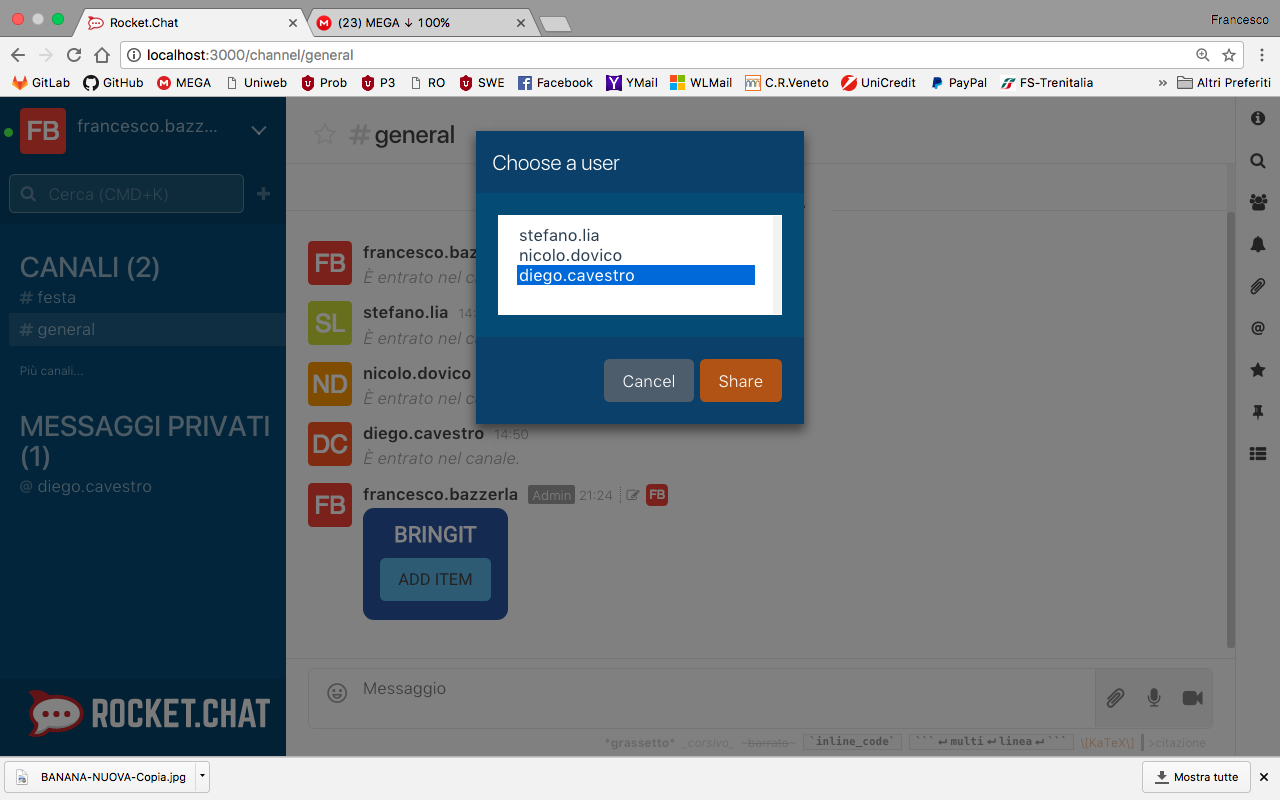
\includegraphics[width=\textwidth]{Sections/3-HowToUse/Images/popup_share_user.png}
  \caption{Popup showing the list of all the users to which is possible sharing a list.}
\end{figure}

Now, select the user you want share the list with and then click on \textit{"Share"}. \\
This will open the following popup, asking you to confirm the sharing action.

\begin{figure}[H]
  \centering 
  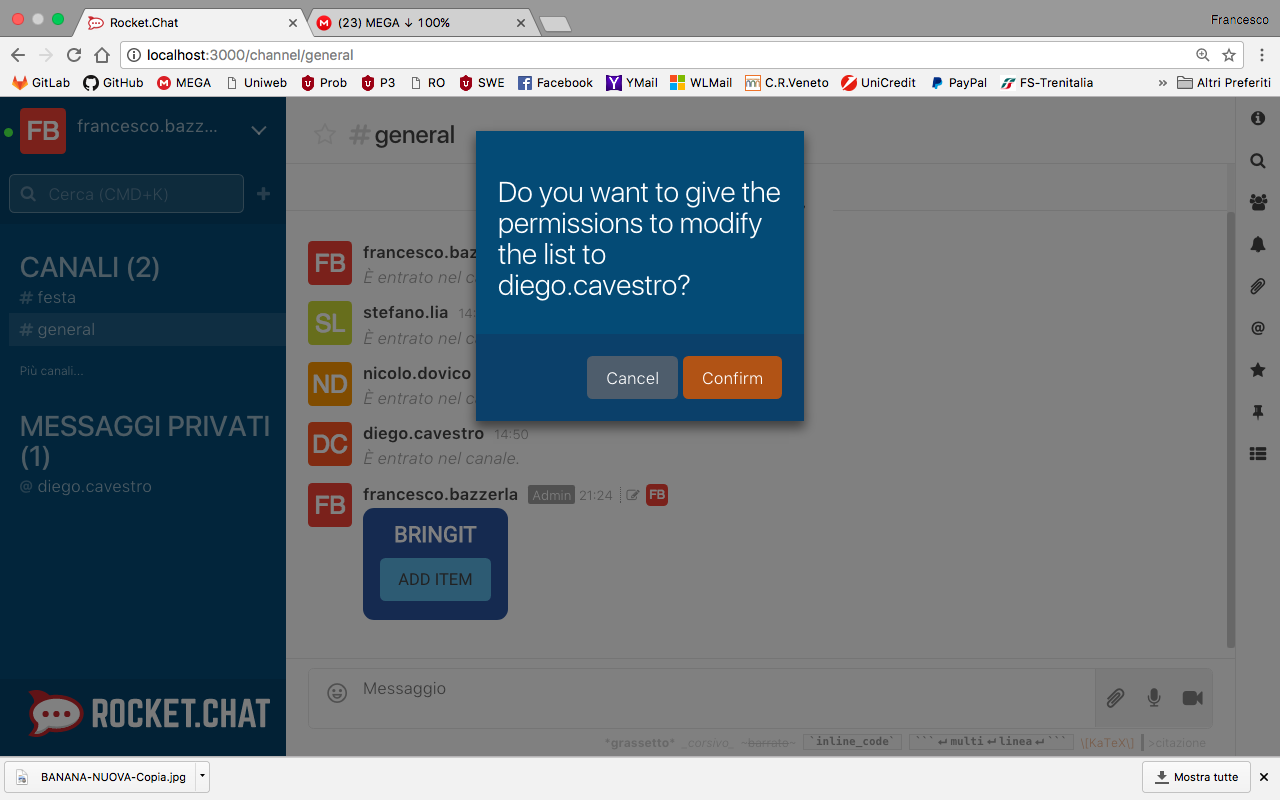
\includegraphics[width=\textwidth]{Sections/3-HowToUse/Images/popup_share_user_confirm.png}
  \caption{Popup to confirm the action to share the list with the selected user.}
\end{figure}

Once you have confirmed the sharing, the bubble will be sent inside the private chat with the user.

\begin{figure}[H]
  \centering 
  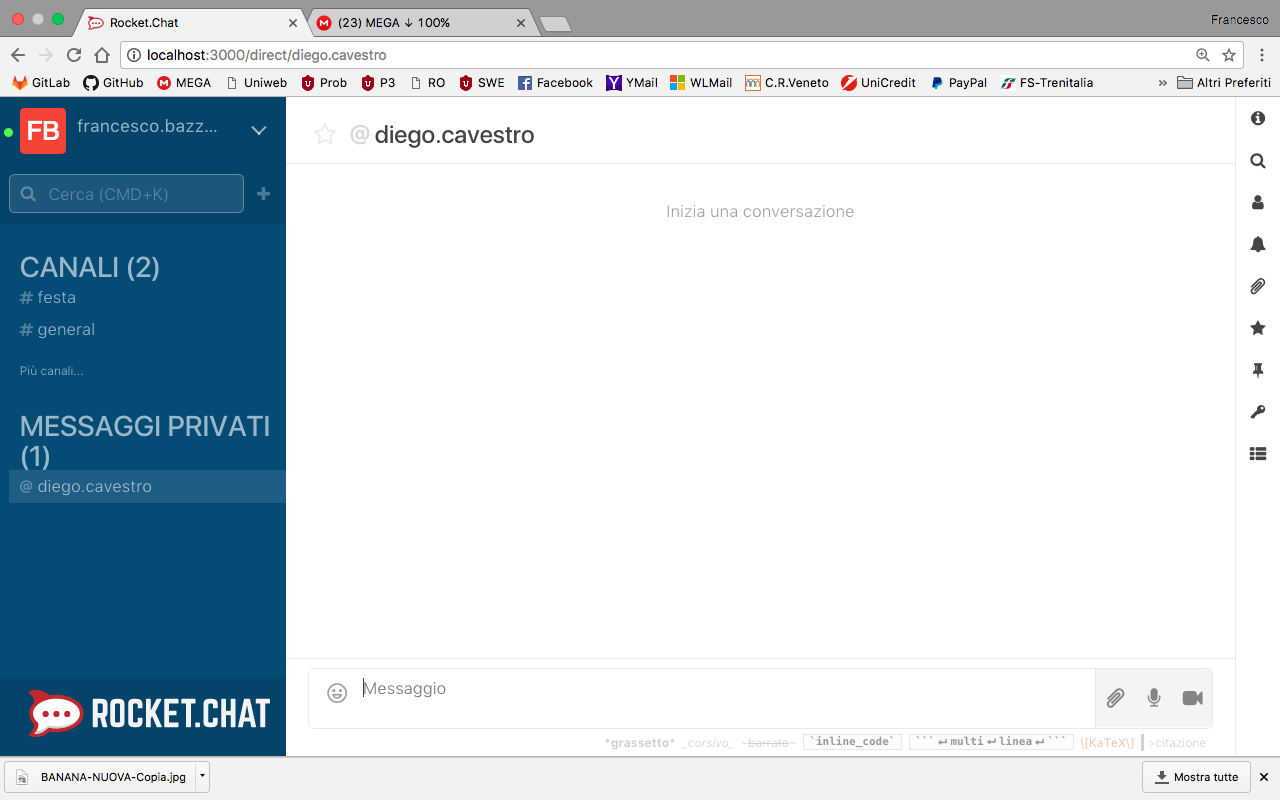
\includegraphics[width=\textwidth]{Sections/3-HowToUse/Images/share_user_before.png}
  \caption{Private chat with a user before sharing the list.}
\end{figure}

\begin{figure}[H]
  \centering 
  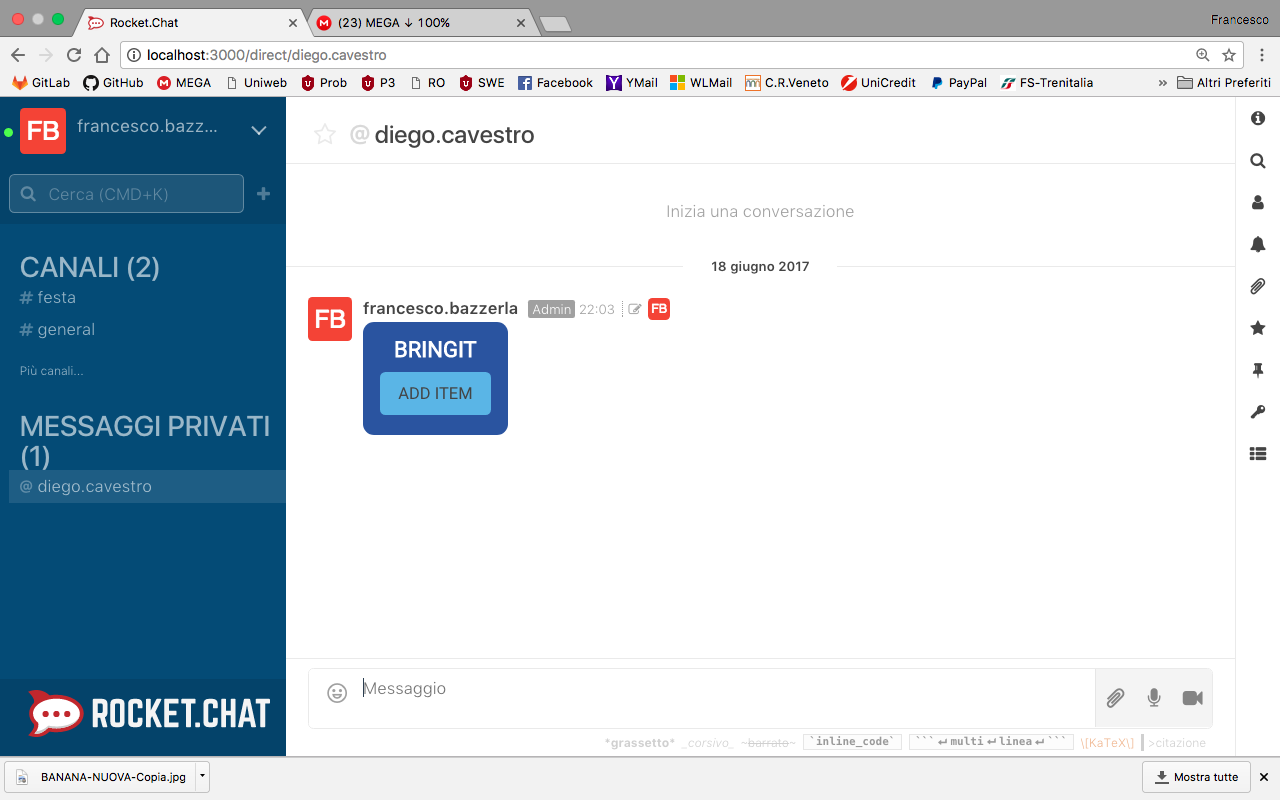
\includegraphics[width=\textwidth]{Sections/3-HowToUse/Images/share_user_after.png}
  \caption{Private chat with a user after sharing the list.}
\end{figure}




\newpage
\subsection{[C] Giving editing permissions to a user}
To add a user from the list of people that have access to the list, just hover above the bubble, and click on the options button.

\begin{figure}[H]
  \centering 
  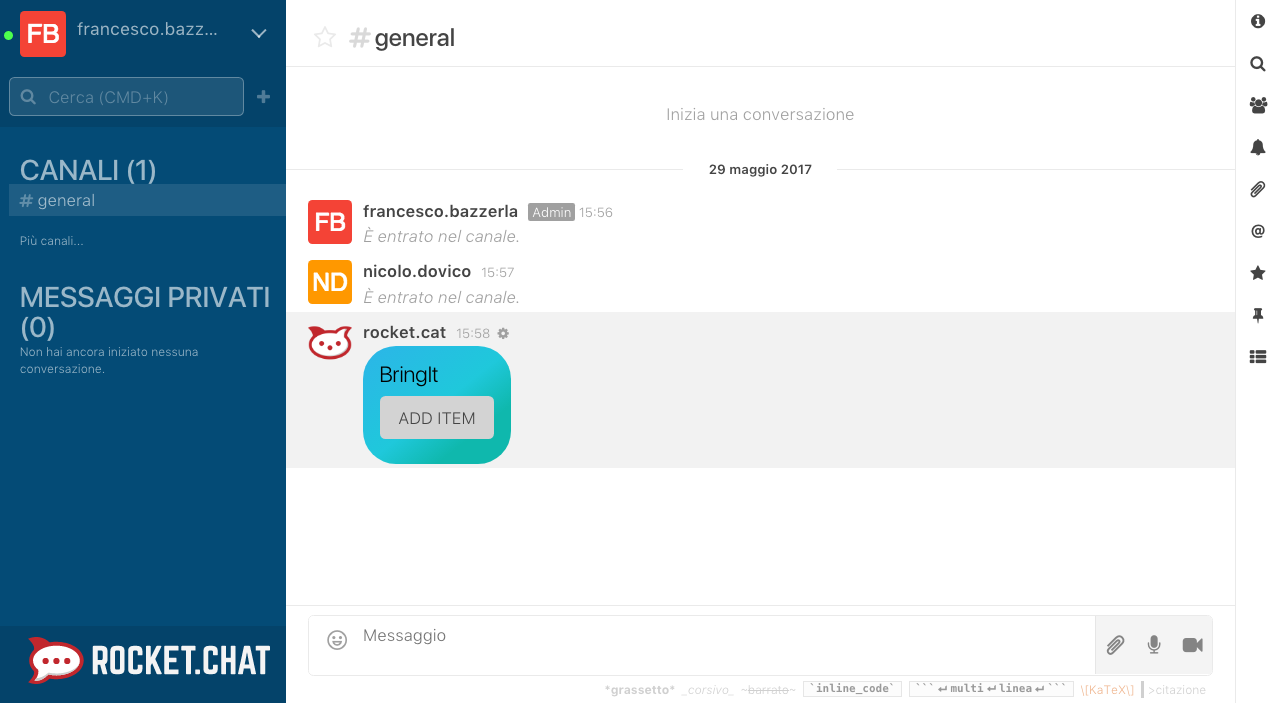
\includegraphics[width=\textwidth]{Sections/3-HowToUse/Images/bubble_options_button.png}
  \caption{Button to show the available list's actions.}
\end{figure}

Select then the button to add the permission to a user.

\begin{figure}[H]
  \centering 
  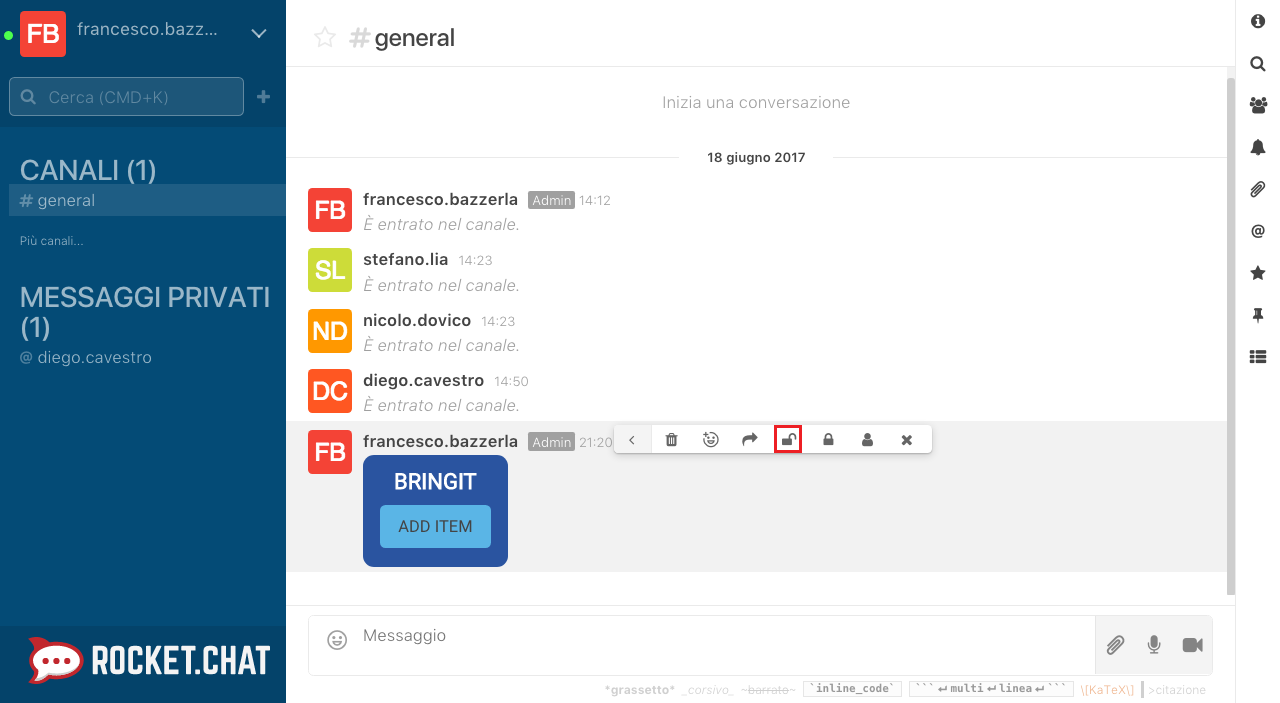
\includegraphics[width=\textwidth]{Sections/3-HowToUse/Images/bubble_option_permission_give.png}
  \caption{Button to remove the permissions of a user.}
\end{figure}

From the popup that opens, select the user(s) you want to add the permission to, and then click on "Ok".

\begin{figure}[H]
  \centering 
  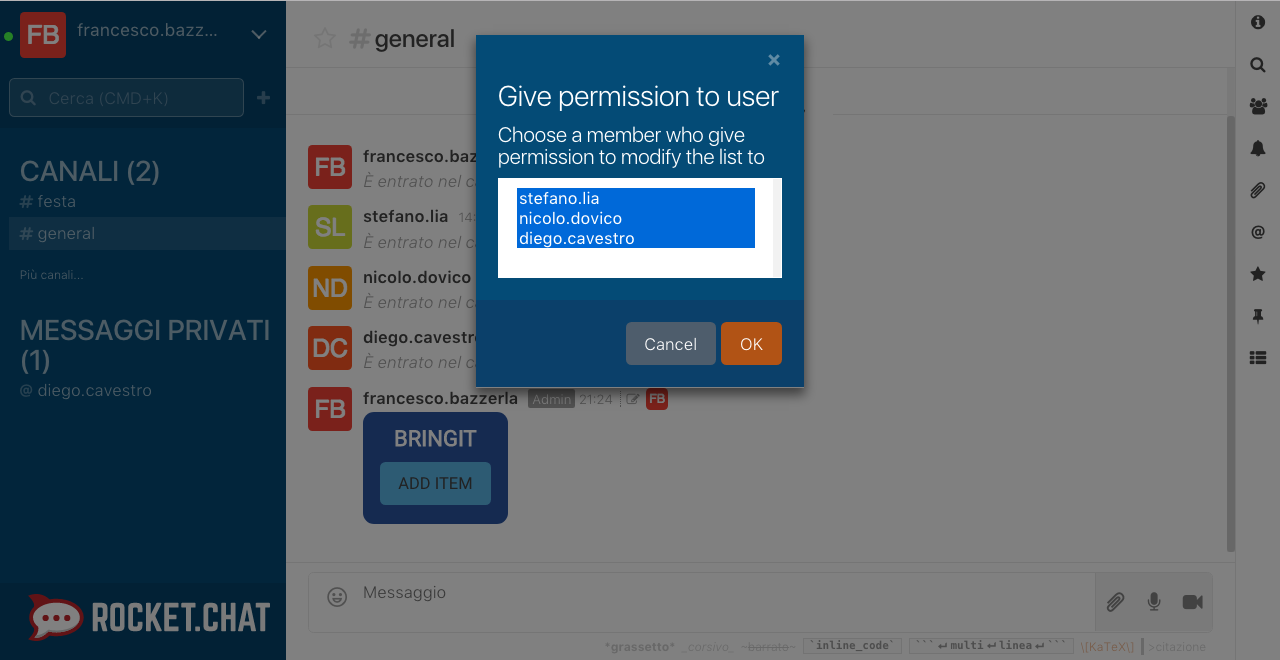
\includegraphics[width=\textwidth]{Sections/3-HowToUse/Images/popup_permission_give.png}
  \caption{Popup to remove the permissions of a user.}
\end{figure}

Note that, if there are no users from which you can remove the permissions, an error will be shown.

\begin{figure}[H]
  \centering 
  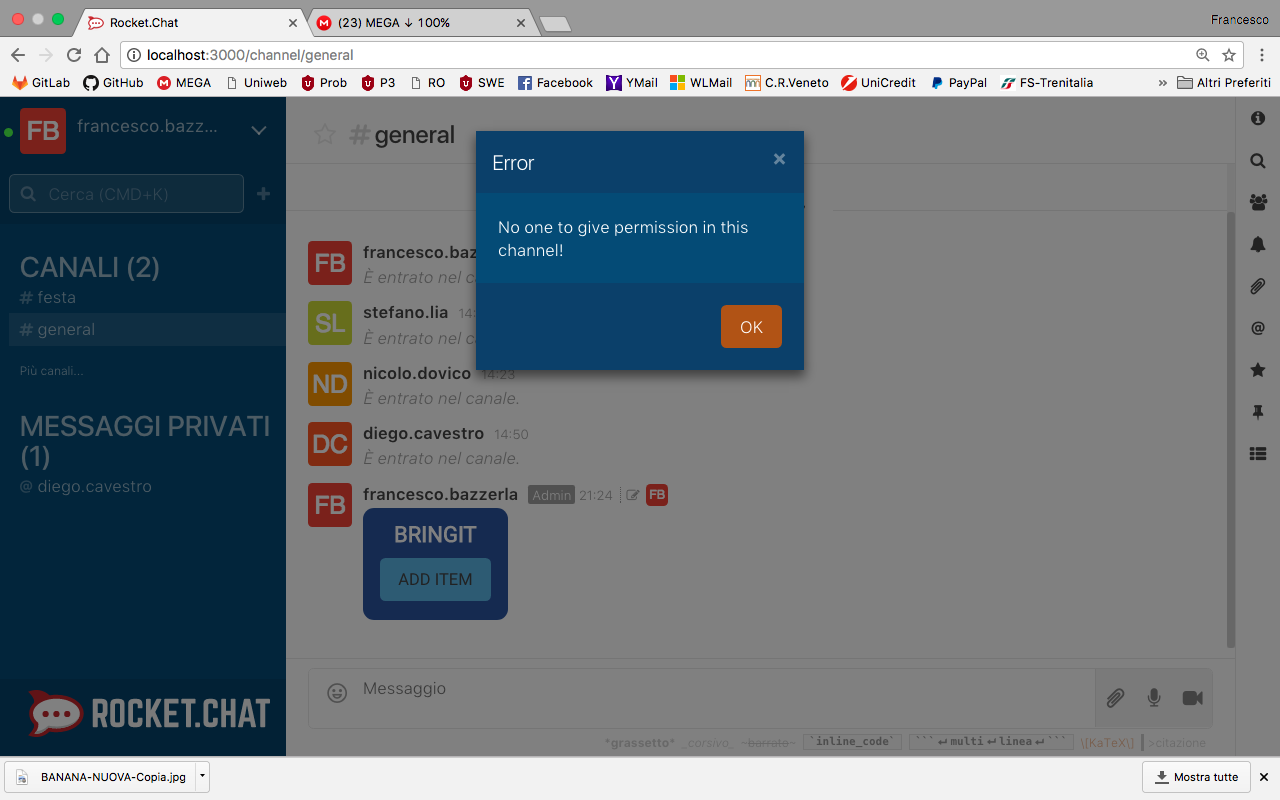
\includegraphics[width=\textwidth]{Sections/3-HowToUse/Images/popup_permission_give_error.png}
  \caption{Error shown if there are no people you can remove the permissions from.}
\end{figure}
\newpage
\subsection{[C] Removing a user}
To remove a user from the list of people that have access to the list, just hover above the bubble, and click on the options button.

\begin{figure}[H]
  \centering 
  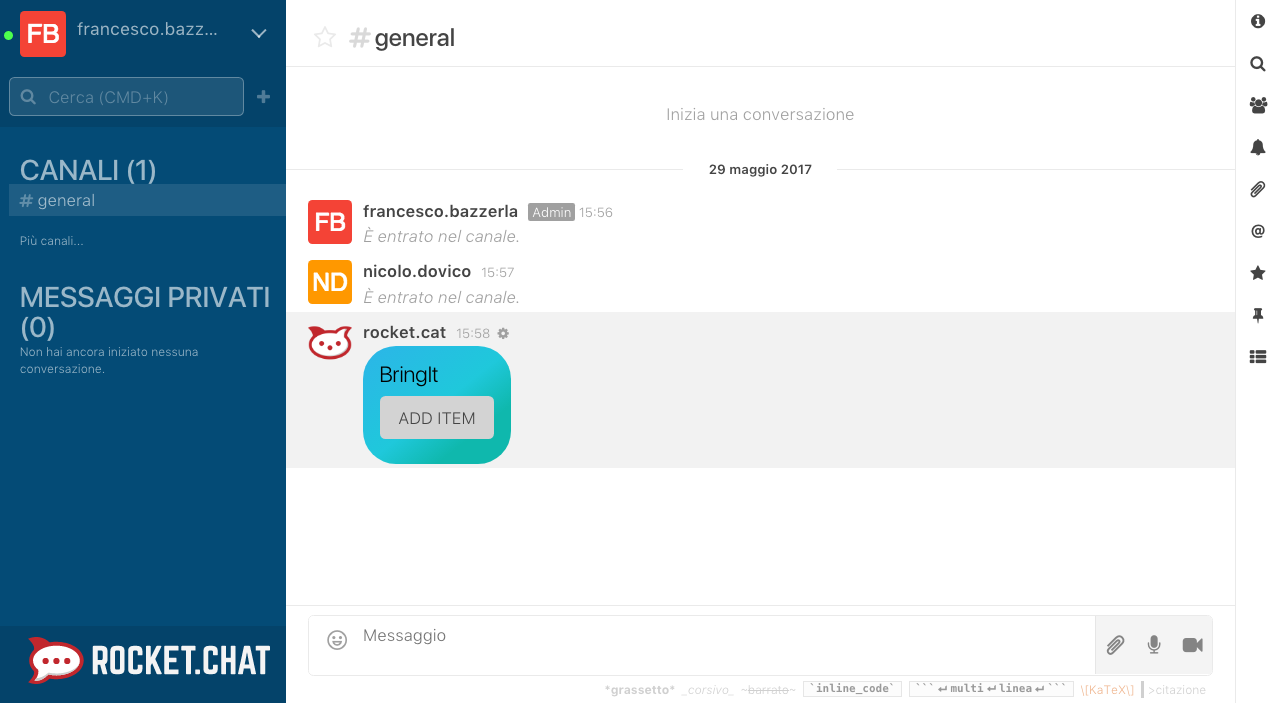
\includegraphics[width=\textwidth]{Sections/3-HowToUse/Images/bubble_options_button.png}
  \caption{Button to show the available list's actions.}
\end{figure}

Select then the button to remove the permissions of a user.

\begin{figure}[H]
  \centering 
  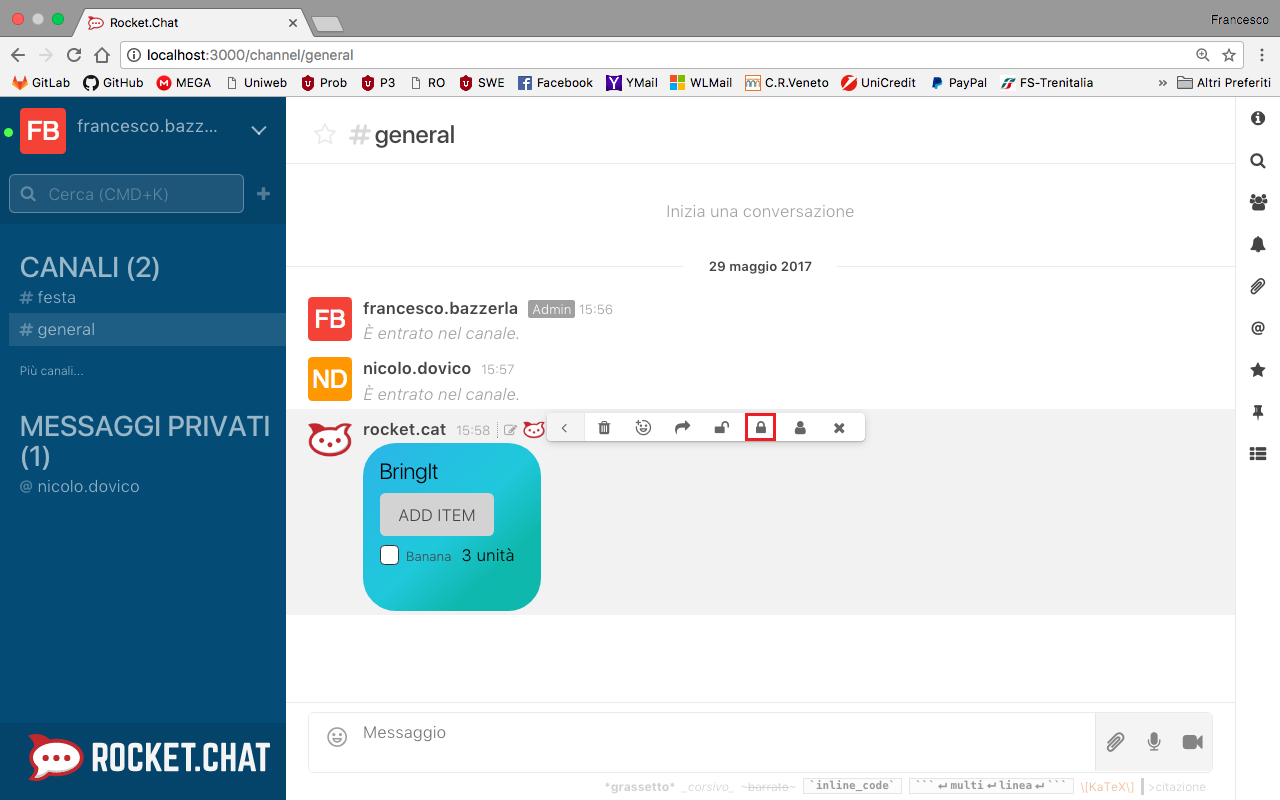
\includegraphics[width=\textwidth]{Sections/3-HowToUse/Images/bubble_option_remove.png}
  \caption{Button to remove the permissions of a user.}
\end{figure}

From the popup that opens, select the user(s) you want to remove the permission from, and then click on "Ok".

\begin{figure}[H]
  \centering 
  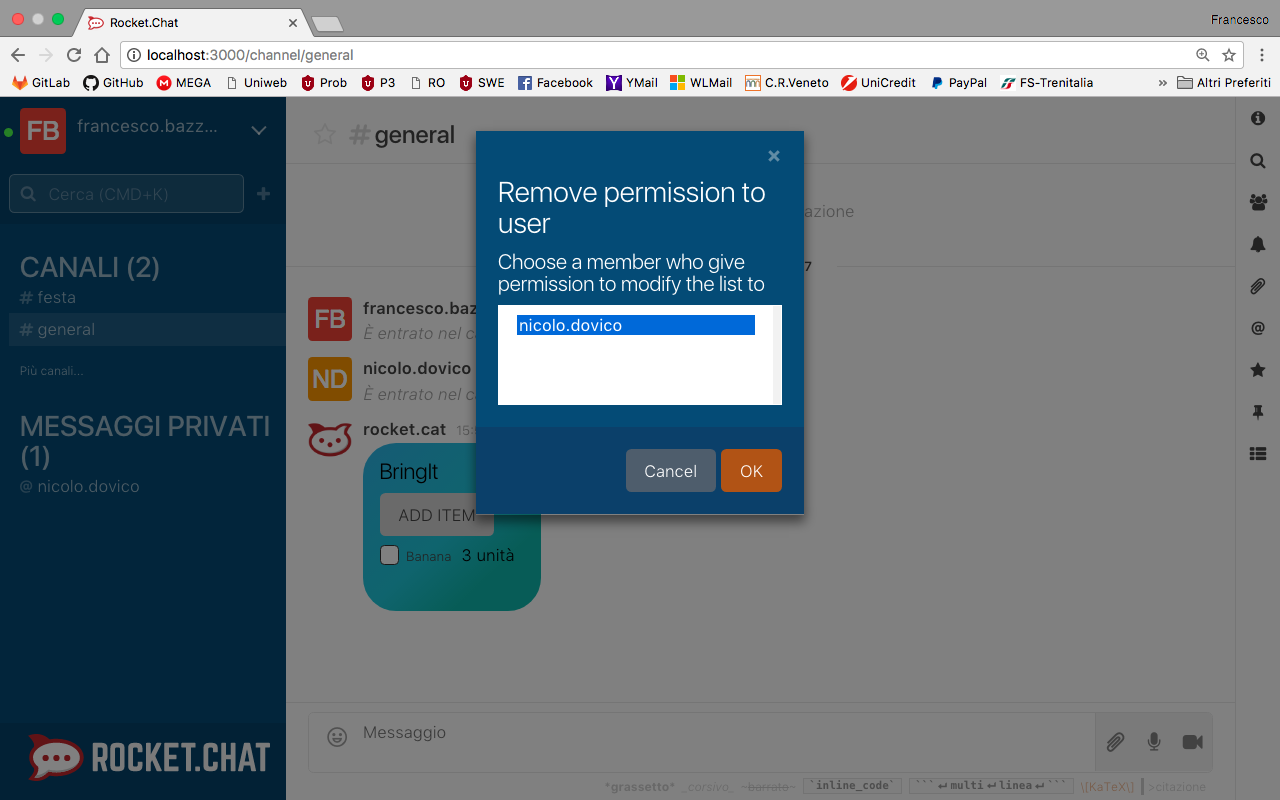
\includegraphics[width=\textwidth]{Sections/3-HowToUse/Images/permission_remove.png}
  \caption{Popup to remove the permissions of a user.}
\end{figure}

Note that, if there are no users from which you can remove the permissions, an error will be shown.

\begin{figure}[H]
  \centering 
  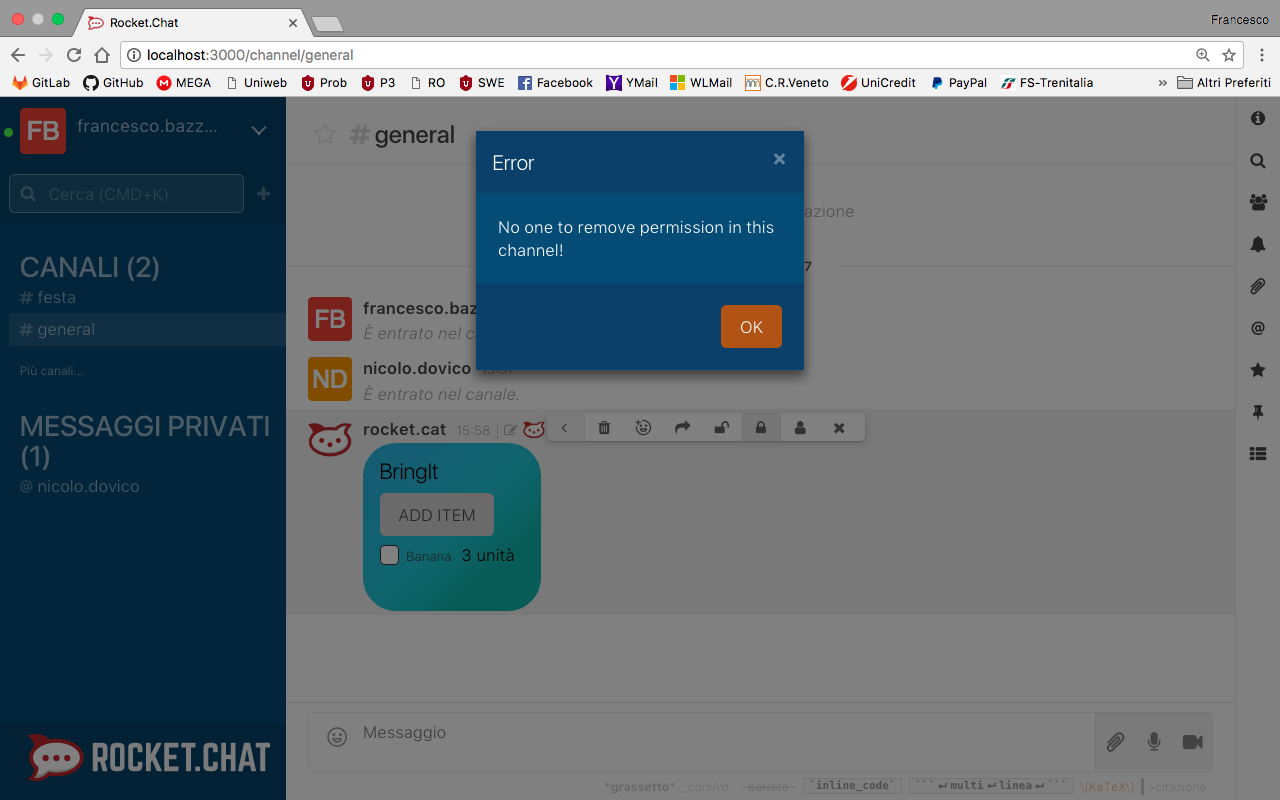
\includegraphics[width=\textwidth]{Sections/3-HowToUse/Images/permission_remove_error.png}
  \caption{Error shown if there are no people you can remove the permissions from.}
\end{figure}
